\chapter{Implementation and discussion} \label{chap: Result}

In this chapter, the results of the performance testing based on assumptions 
and two industrial use cases to verify the feasibility of the methods presented 
in chapter \ref{chap: Meth} will be discussed. The tests will be divided into 
two parts: internal (section \ref{chap: Result-Internal}) and 
external (section \ref{chap: Result-External}), as previously mentioned in 
chapter \ref{chap: Meth}.



\section{Internal}\label{chap: Result-Internal}
In the following sections, multiple tests are conducted on the agent communication system 
of the internal \gls{mas}. These tests involve passing messages through the \gls{ca} under 
WebSocket architecture. The results of these tests are discussed in 
section \ref{chap: Result-WS}. In addition to testing the performance of WebSocket 
architecture alone, a comparison between WebSocket and \gls{http} is done to verify 
the feasibility of WebSocket. Packet prioritization tests will also be performed in 
section \ref{chap: Result-priority}. Finally, the test results of the 
WebSocket-based \gls{mas} architecture under the BMW use case are presented to 
close the sections.


\subsection{Test results of WebSocket in various performance testing including worst case scenarios} \label{chap: Result-WS}

After the construction a \gls{mas} under WebSocket, the speed, robustness, 
reliability and application size of the system will be examined by 
performance tests. 

\subsubsection{Increasing client numbers}
In the real world, the number of clients will significantly influence the server's 
performance. Assume all agents serve as clients and \gls{ca} as a central server. 
By handling an increasing number of connection requests and the growing demands of 
data processing capacity, the average total delay with or without process time can 
be roughly described as an overall increasing pattern. However, it does not necessarily 
need to be linear based on several reasons. In exercise, concurrent programming will 
speed up the processing for a significant computation problem. As depicted in 
fig.\ref{fig: proportional-clients}, the average process time from one to ten clients 
decreases with better utilization of the \gls{cpu} power due to concurrent processing. 
However, by further increasing the clients' number, the speedup will be limited 
by \gls{cpu} cores number. Assume that a \gls{cpu} has eight cores, and each core 
can handle two threads. It will have a total of 16 threads to perform tasks. In the 
WebSocket-based \gls{mas} program, the asynchronous I/O framework asyncio is used 
to handle the execution of the coroutine in order to utilize the threads' power 
better.
Therefore, asyncio is more suitable for larger computational tasks than synchronous 
single-thread programming.

It appears that there is a limit on the number of clients that the system can handle 
to prevent it from breaking down. When a single server handles all clients, the 
server experiences a timeout problem when the number of clients reaches 1000. 
Therefore, distributing clients across more servers could be a possible solution 
to this issue.


\begin{figure}[htb]
    \begin{subfigure}[b]{0.49\textwidth}
        \centering
        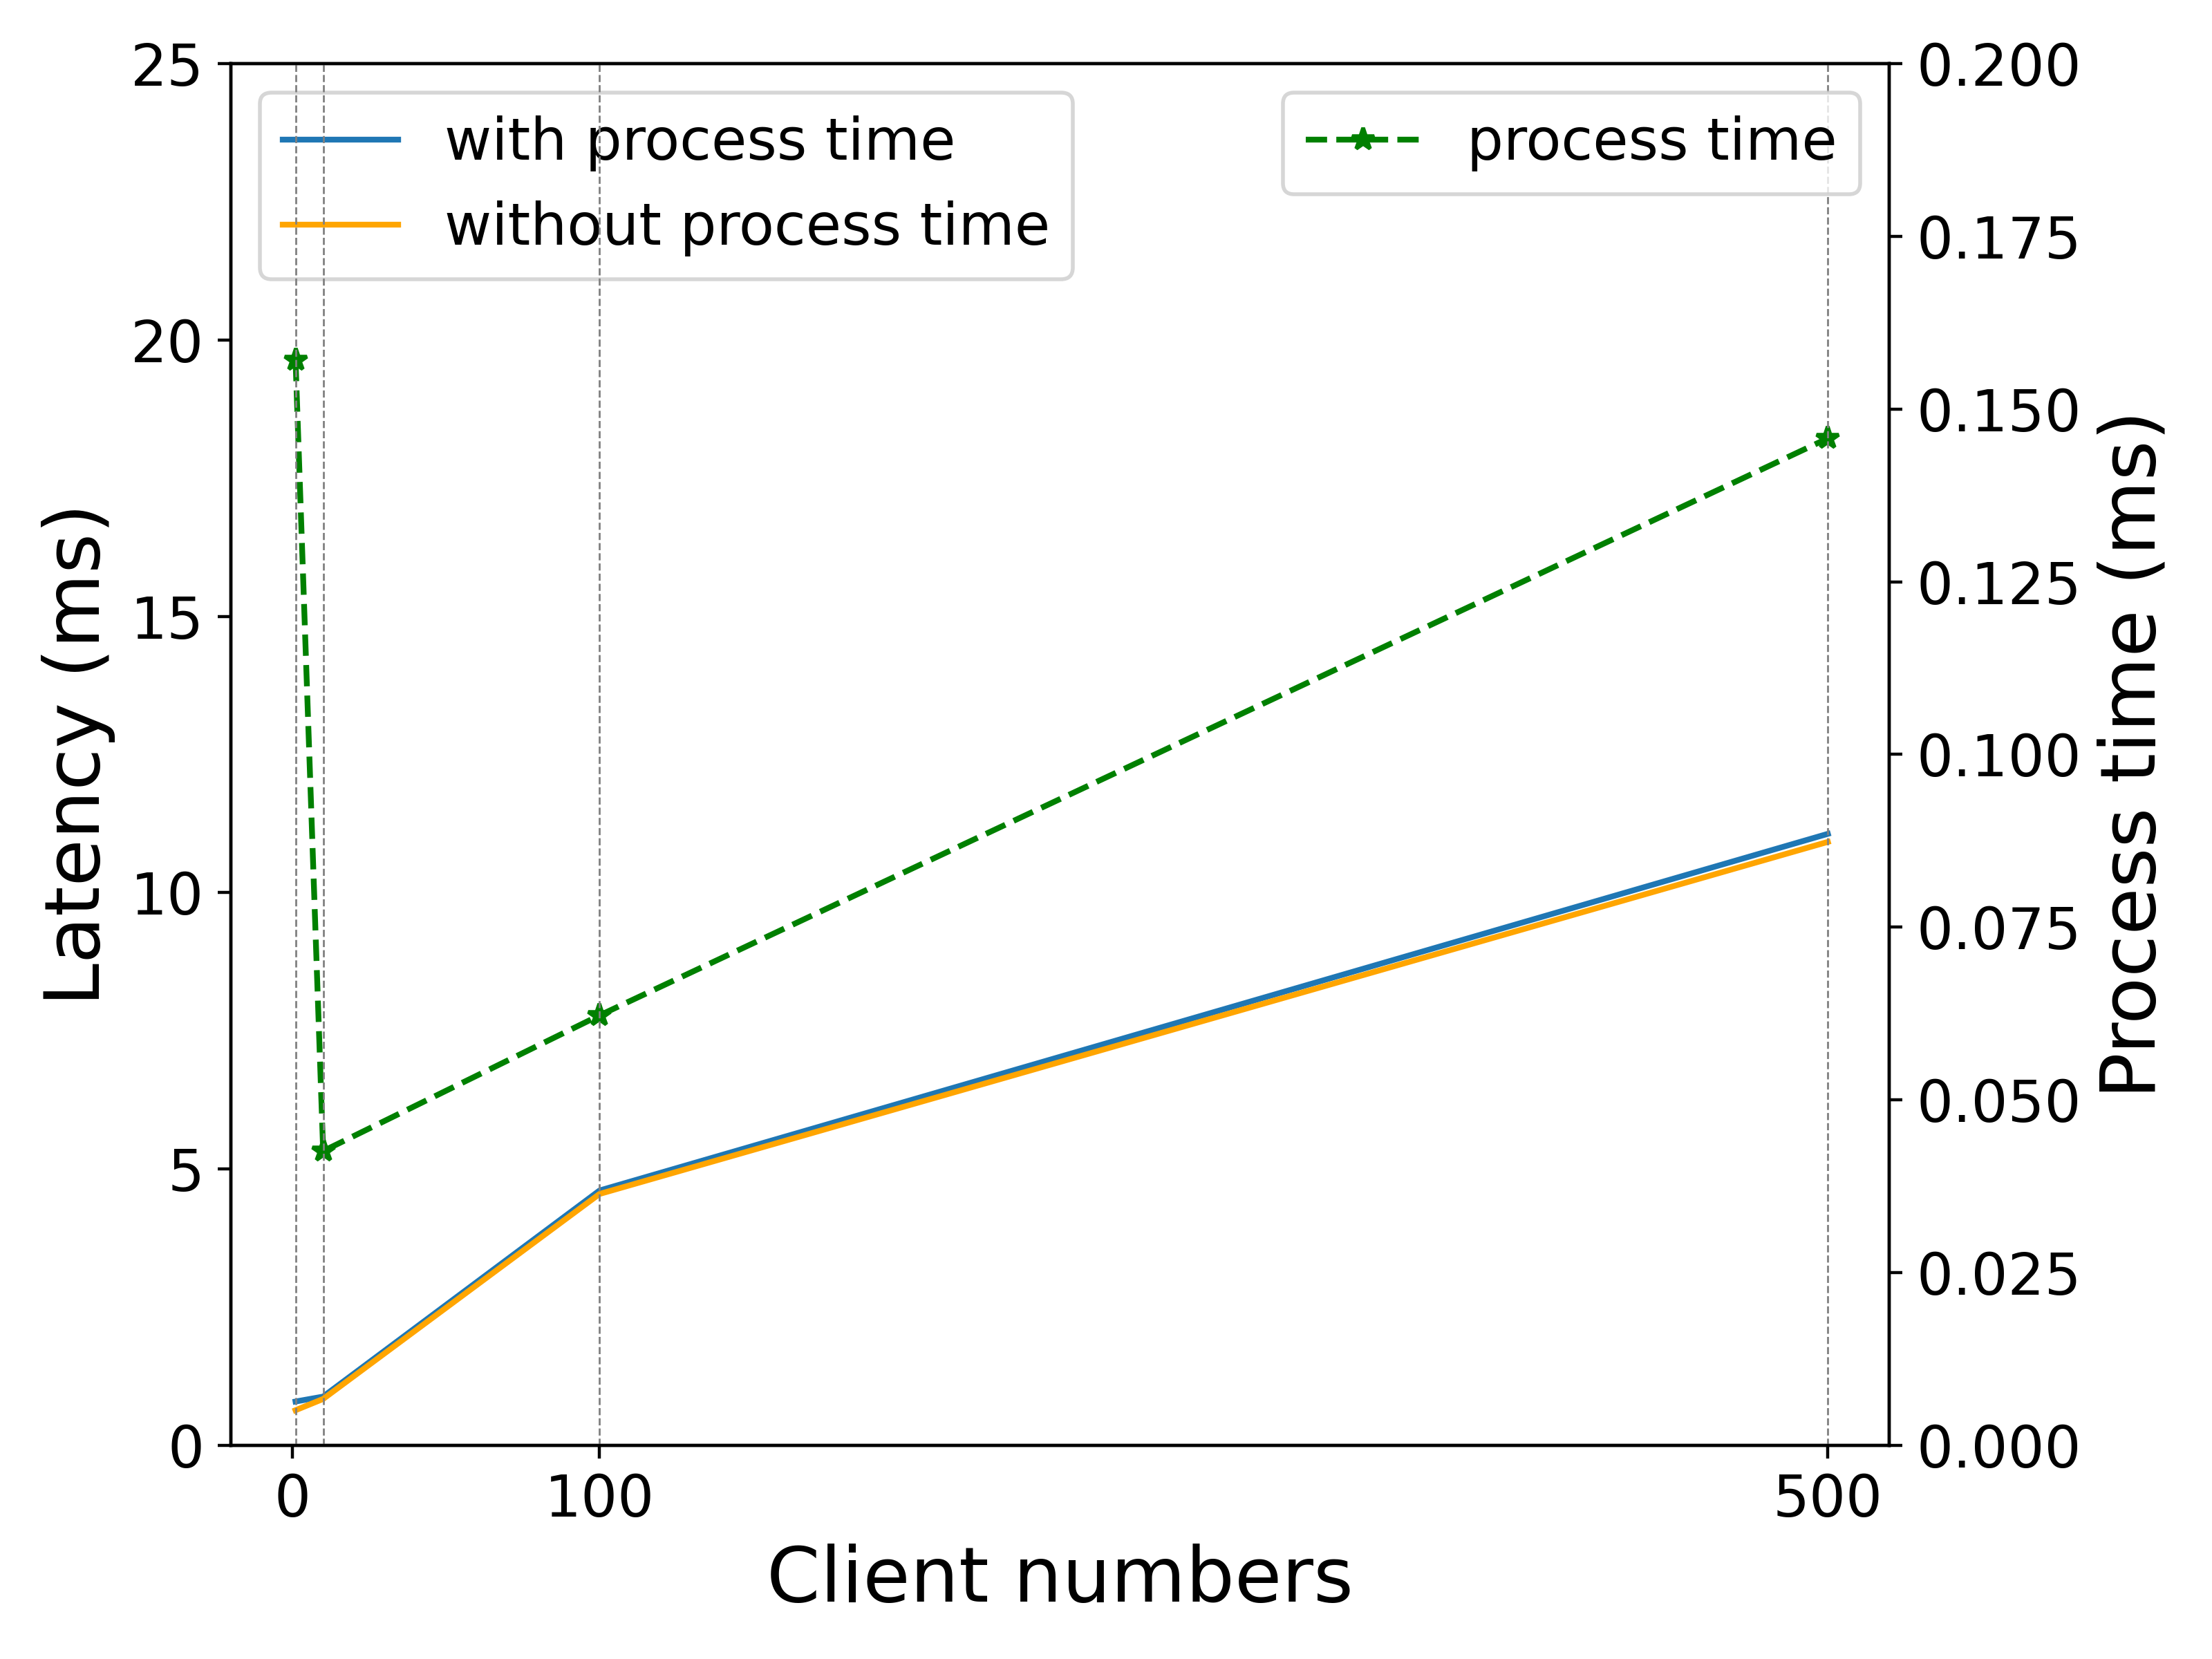
\includegraphics[width=\textwidth]{figures/tests/proportional_tests/Average_string_messages_sending_time_of_100_tests_of_diff_client_numbers.png}\hfill 
        \caption{} \label{fig: proportional-clients-a}
    \end{subfigure}
    \begin{subfigure}[b]{0.49\textwidth}
        \centering
        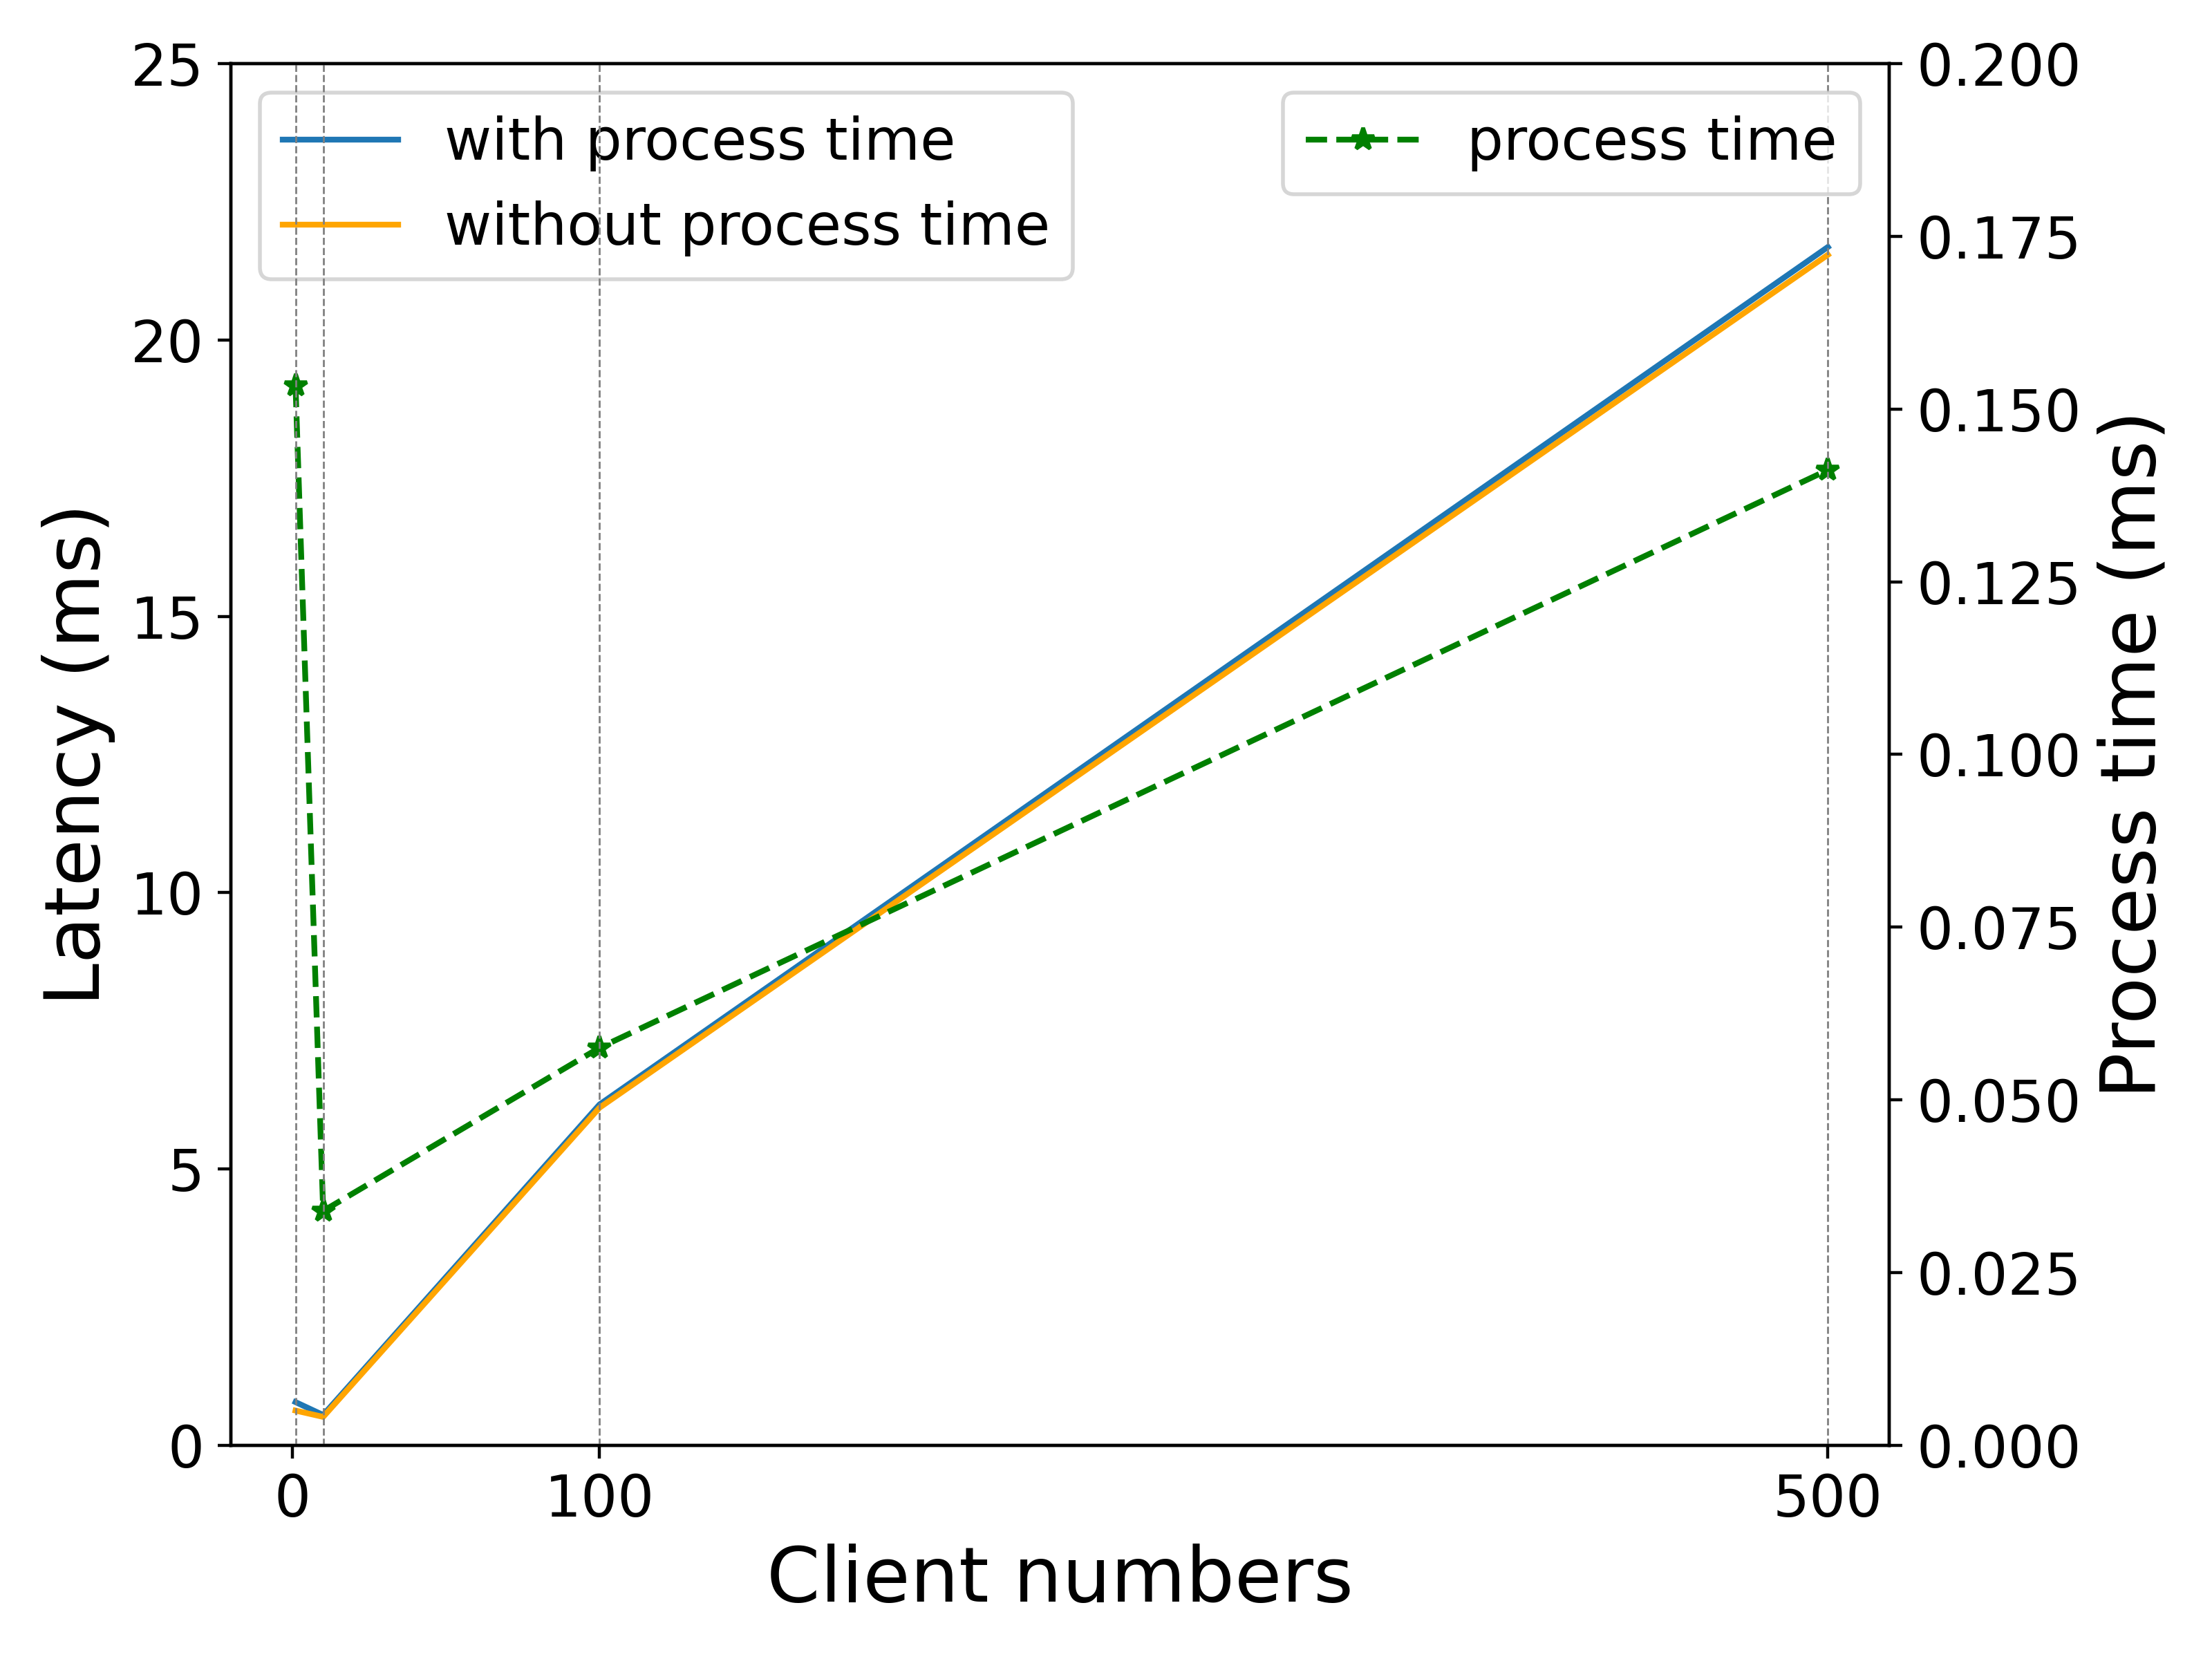
\includegraphics[width=\textwidth]{figures/tests/proportional_tests/Average_string_messages_receiving_time_of_100_tests_of_diff_client_numbers.png}\hfill 
        \caption{} \label{fig: proportional-clients-b}
        \end{subfigure}

    \caption{Average delay of sending a string message 100 times 
    to a clientR from 1, 10, 100 or 500 clients separately. (a) Messages sent forward, 
    and (b) response messages from clientR. 
    \label{fig: proportional-clients}}
\end{figure}


\subsubsection{Increasing server numbers}
When 1000 clients are communicating with clientR, their messages will be split 
into two or three groups and routed through different servers due to system 
limitations. According to fig.\ref{fig: NSConceptual}, only a maximum of three 
servers can be used for the test, as per the hardware configuration of the external 
routing solutions. However, we can make some assumptions based on the results 
shown in fig.\ref{fig: proportional-servers}.


\begin{figure}[htb]
    \centering
    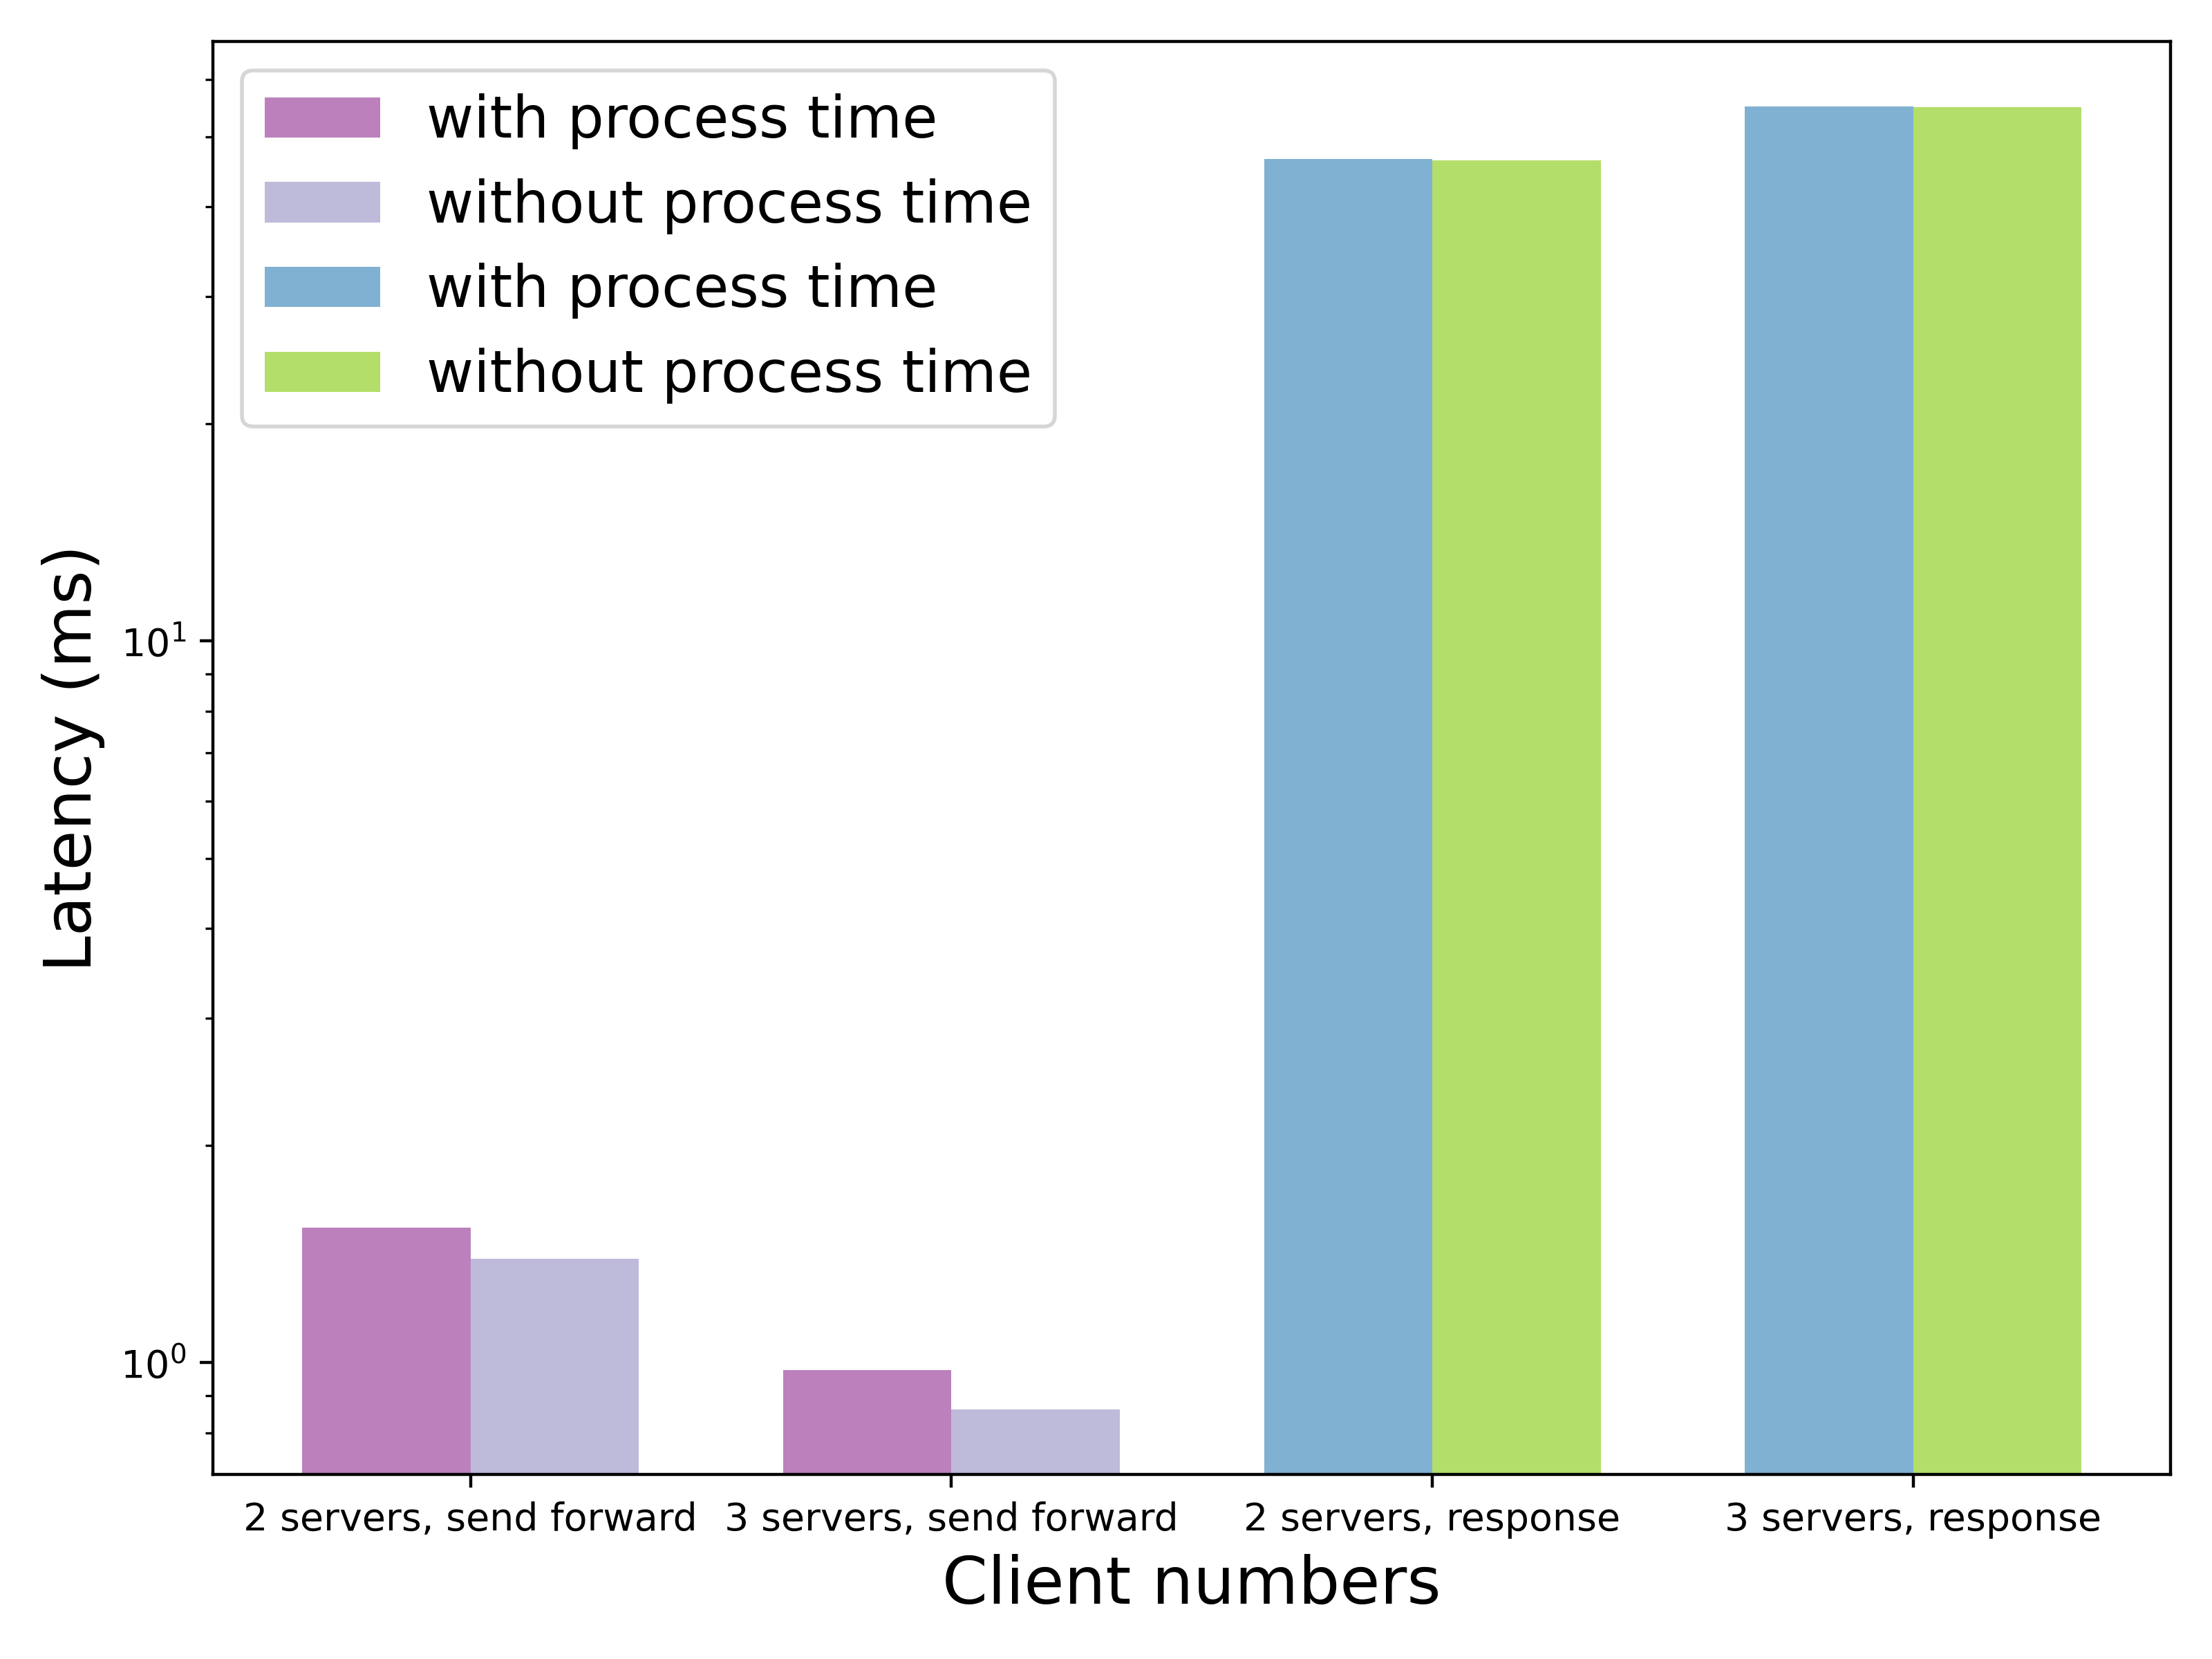
\includegraphics[width=0.8\textwidth]{figures/tests/proportional_tests/Average_string_messages_receiving_time_of_100_tests_diff_server_numbers.png}\hfill 
    \caption{Average delay of sending a string message 100 times 
    to a clientR from 1000 clients through 2 or 3 servers separately. 
    \label{fig: proportional-servers}}
\end{figure}

The figure shown in fig.\ref{fig: proportional-servers} indicates that introducing 
additional servers to the system results in a reduction of latency. This means that 
limited productive resources can be better utilized for frequent client interactions. 
However, the latency of response messages from clientR is unexpectedly higher 
in fig.\ref{fig: proportional-servers}. This could be due to high \gls{cpu} consumption. 
When multiple servers are running on the same device, the send and receive processes 
in the WebSocket are operated separately. Due to the high occupation of \gls{cpu} power, 
the loads between each process might be unbalanced and added up by the increment of servers.

\subsubsection{Increasing string message length}\label{chap: Result-Internal-string}
To determine the effect of packet size (i.e., message length) on system performance, 
it's important to conduct another significant test. The formula for packet transmission 
time is given as:


\begin{equation}
    Transmission $ $ delay = Packet $ $ size/Bandwidth
\end{equation}

Assuming the bandwidth is constant, the transmission time should be linearly proportional 
to an increasing packet size. In fig.\ref{fig: proportional-stringsize}, various string 
message lengths ranging from 1KB to 10MB are compared, indicating the linear dependency 
of latency and string size in both forward (fig.\ref{fig: proportional-stringsize-a}) 
and return message (fig.\ref{fig: proportional-stringsize-b}). This confirms the 
transmission time formula. Additionally, it's worth noting that the server's process 
time increases with the size of the message bytes. In real-world scenarios, large string 
messages should be broken down into smaller parts for communication, significantly 
reducing process time consumption. To examine system limits, a string with a size of 
up to 100MB is tested, resulting in a system timeout error that exceeds the server's 
maximum processing capacity.

\begin{figure}[htb]
    \begin{subfigure}{0.49\textwidth}
        \centering
        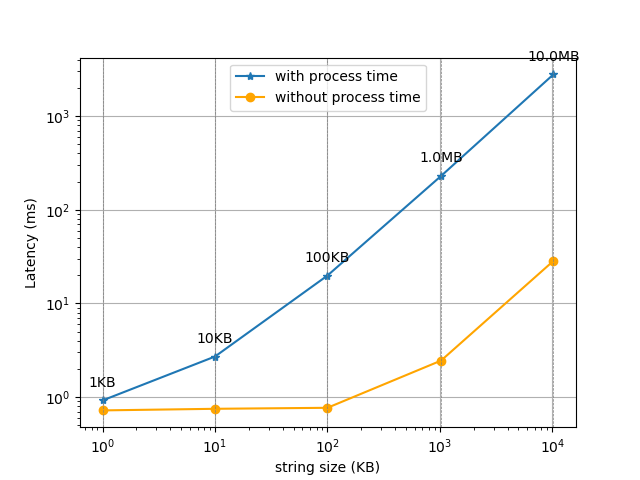
\includegraphics[width=\textwidth]{figures/tests/proportional_tests/log_Average_string_messages_sending_time_of_100_tests_1KB_to_10MB.png}
        \caption{} \label{fig: proportional-stringsize-c}
    \end{subfigure}
    \begin{subfigure}{0.49\textwidth}
        \centering
        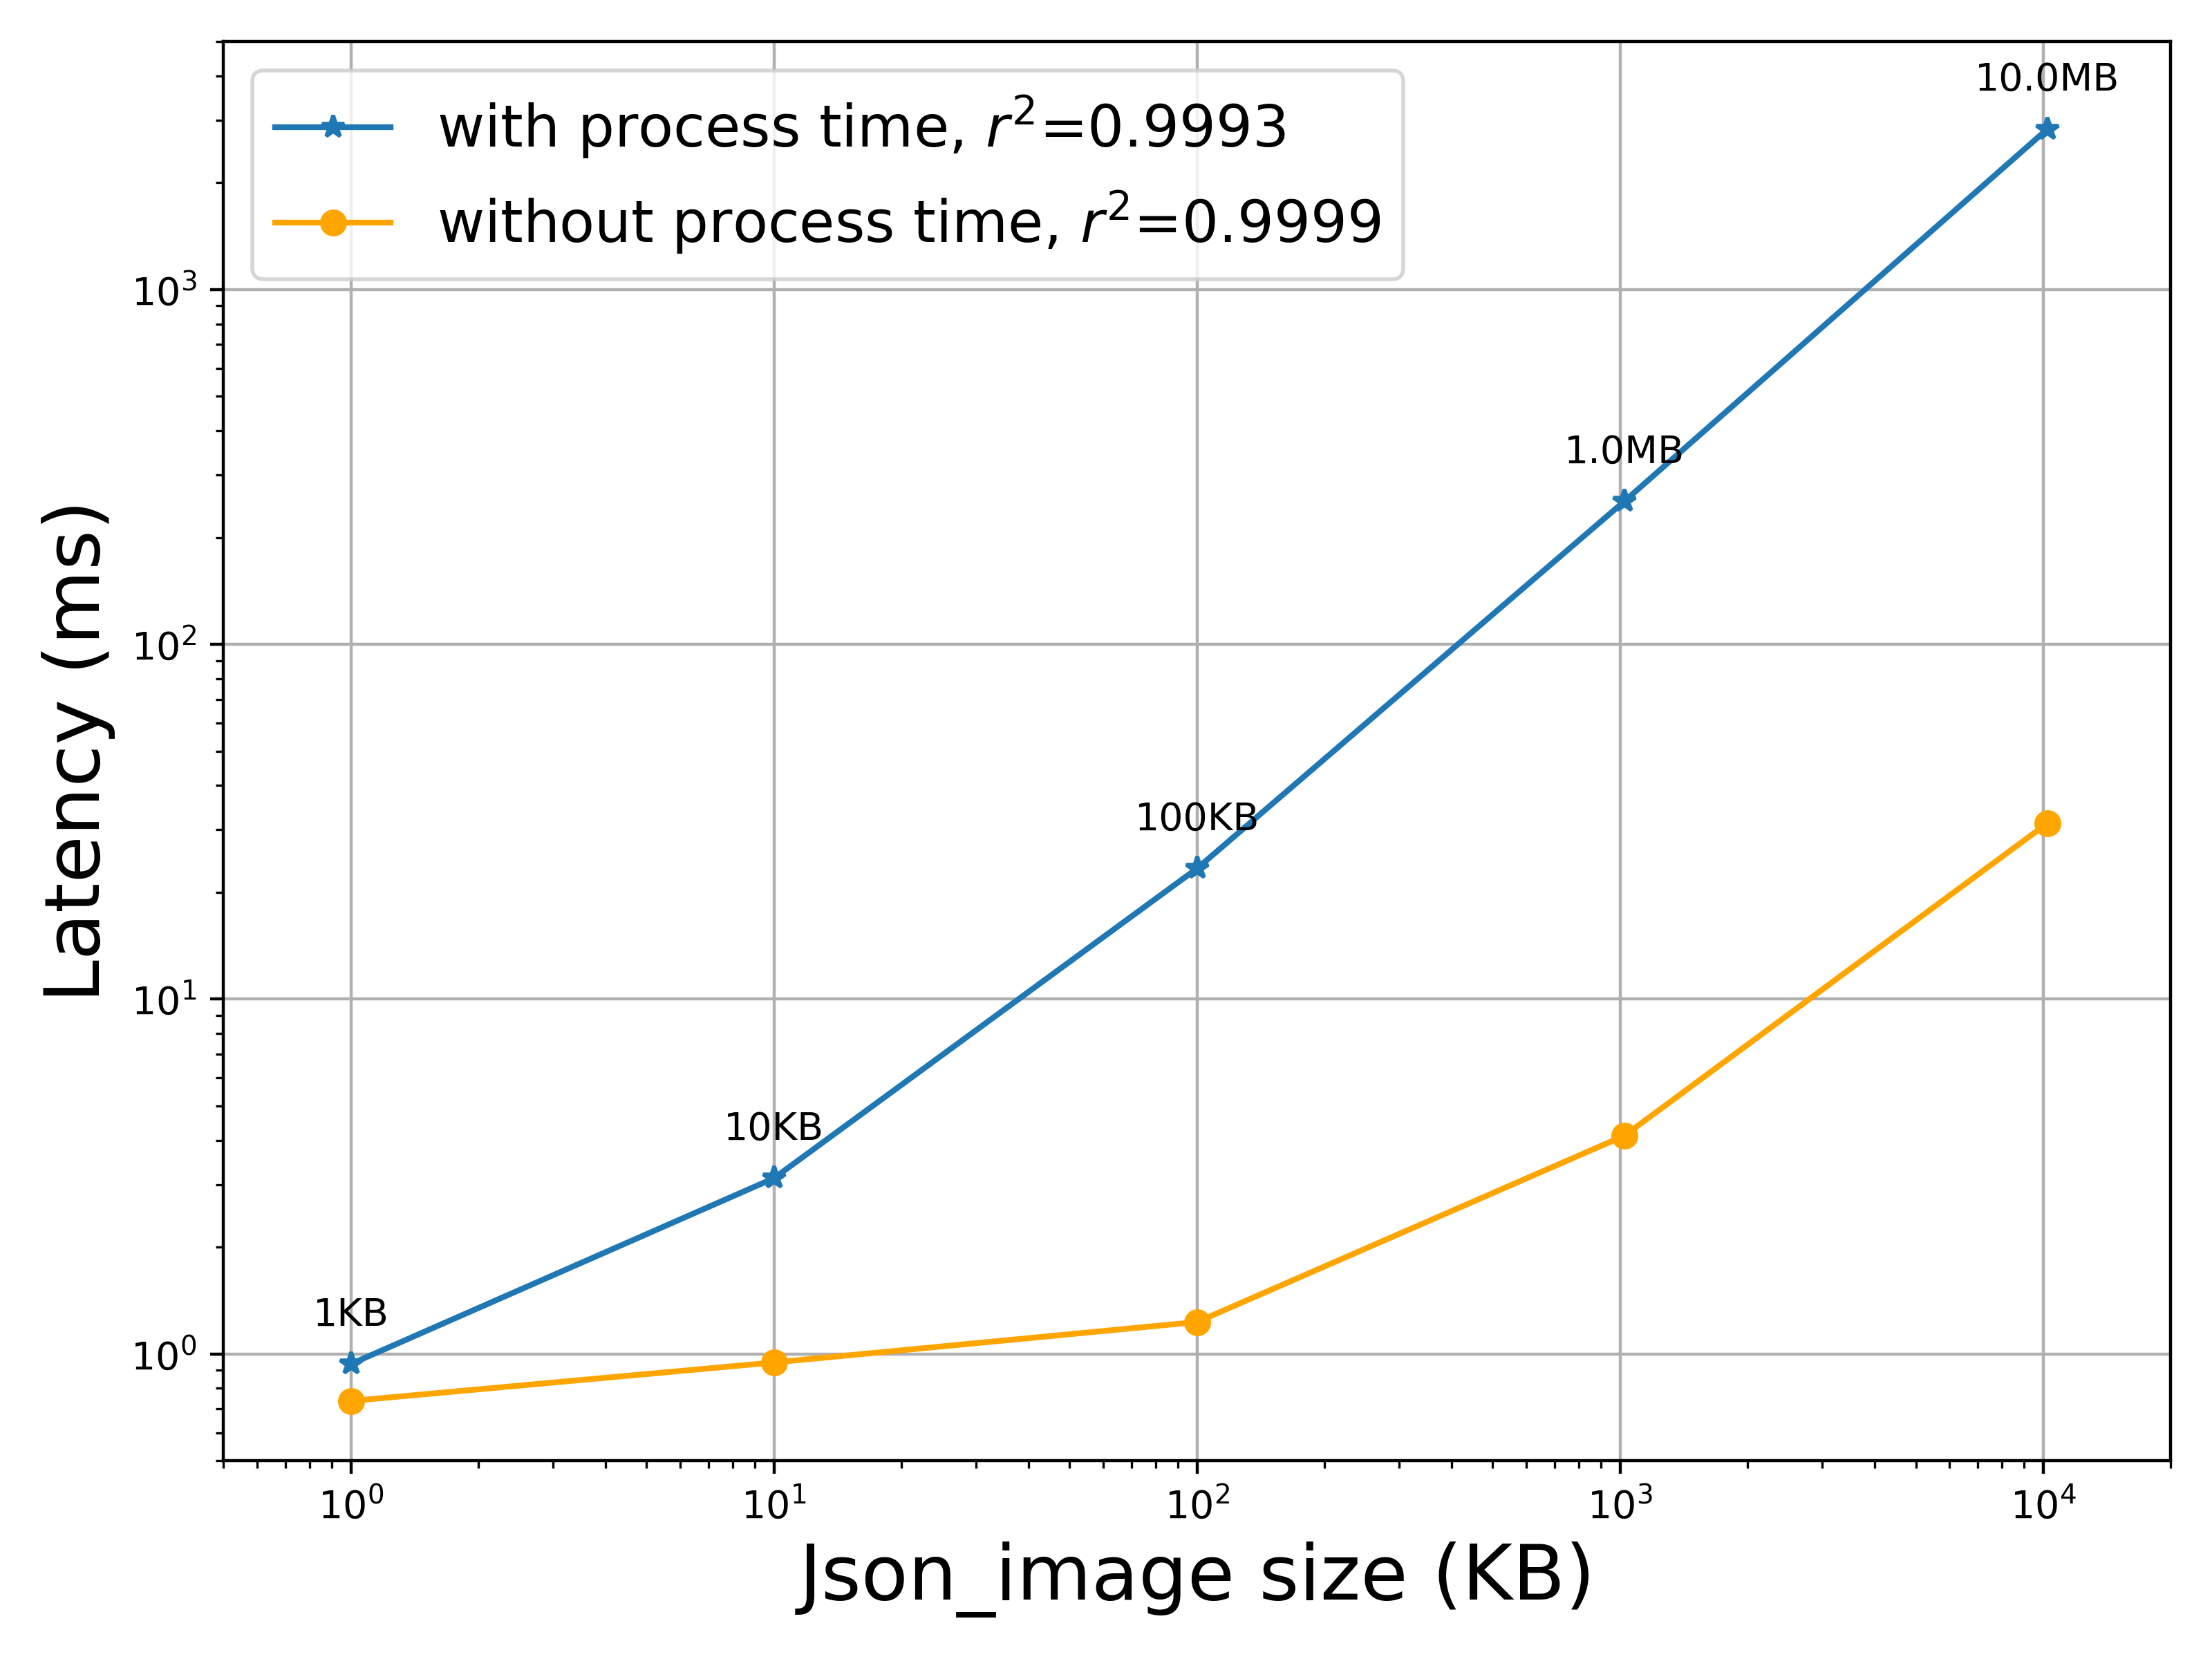
\includegraphics[width=\textwidth]{figures/tests/proportional_tests/log_Average_string_messages_receiving_time_of_100_tests_1KB_to_10MB.png}
        \caption{} \label{fig: proportional-stringsize-d}
    \end{subfigure}

    \begin{subfigure}{0.49\textwidth}
        \centering
        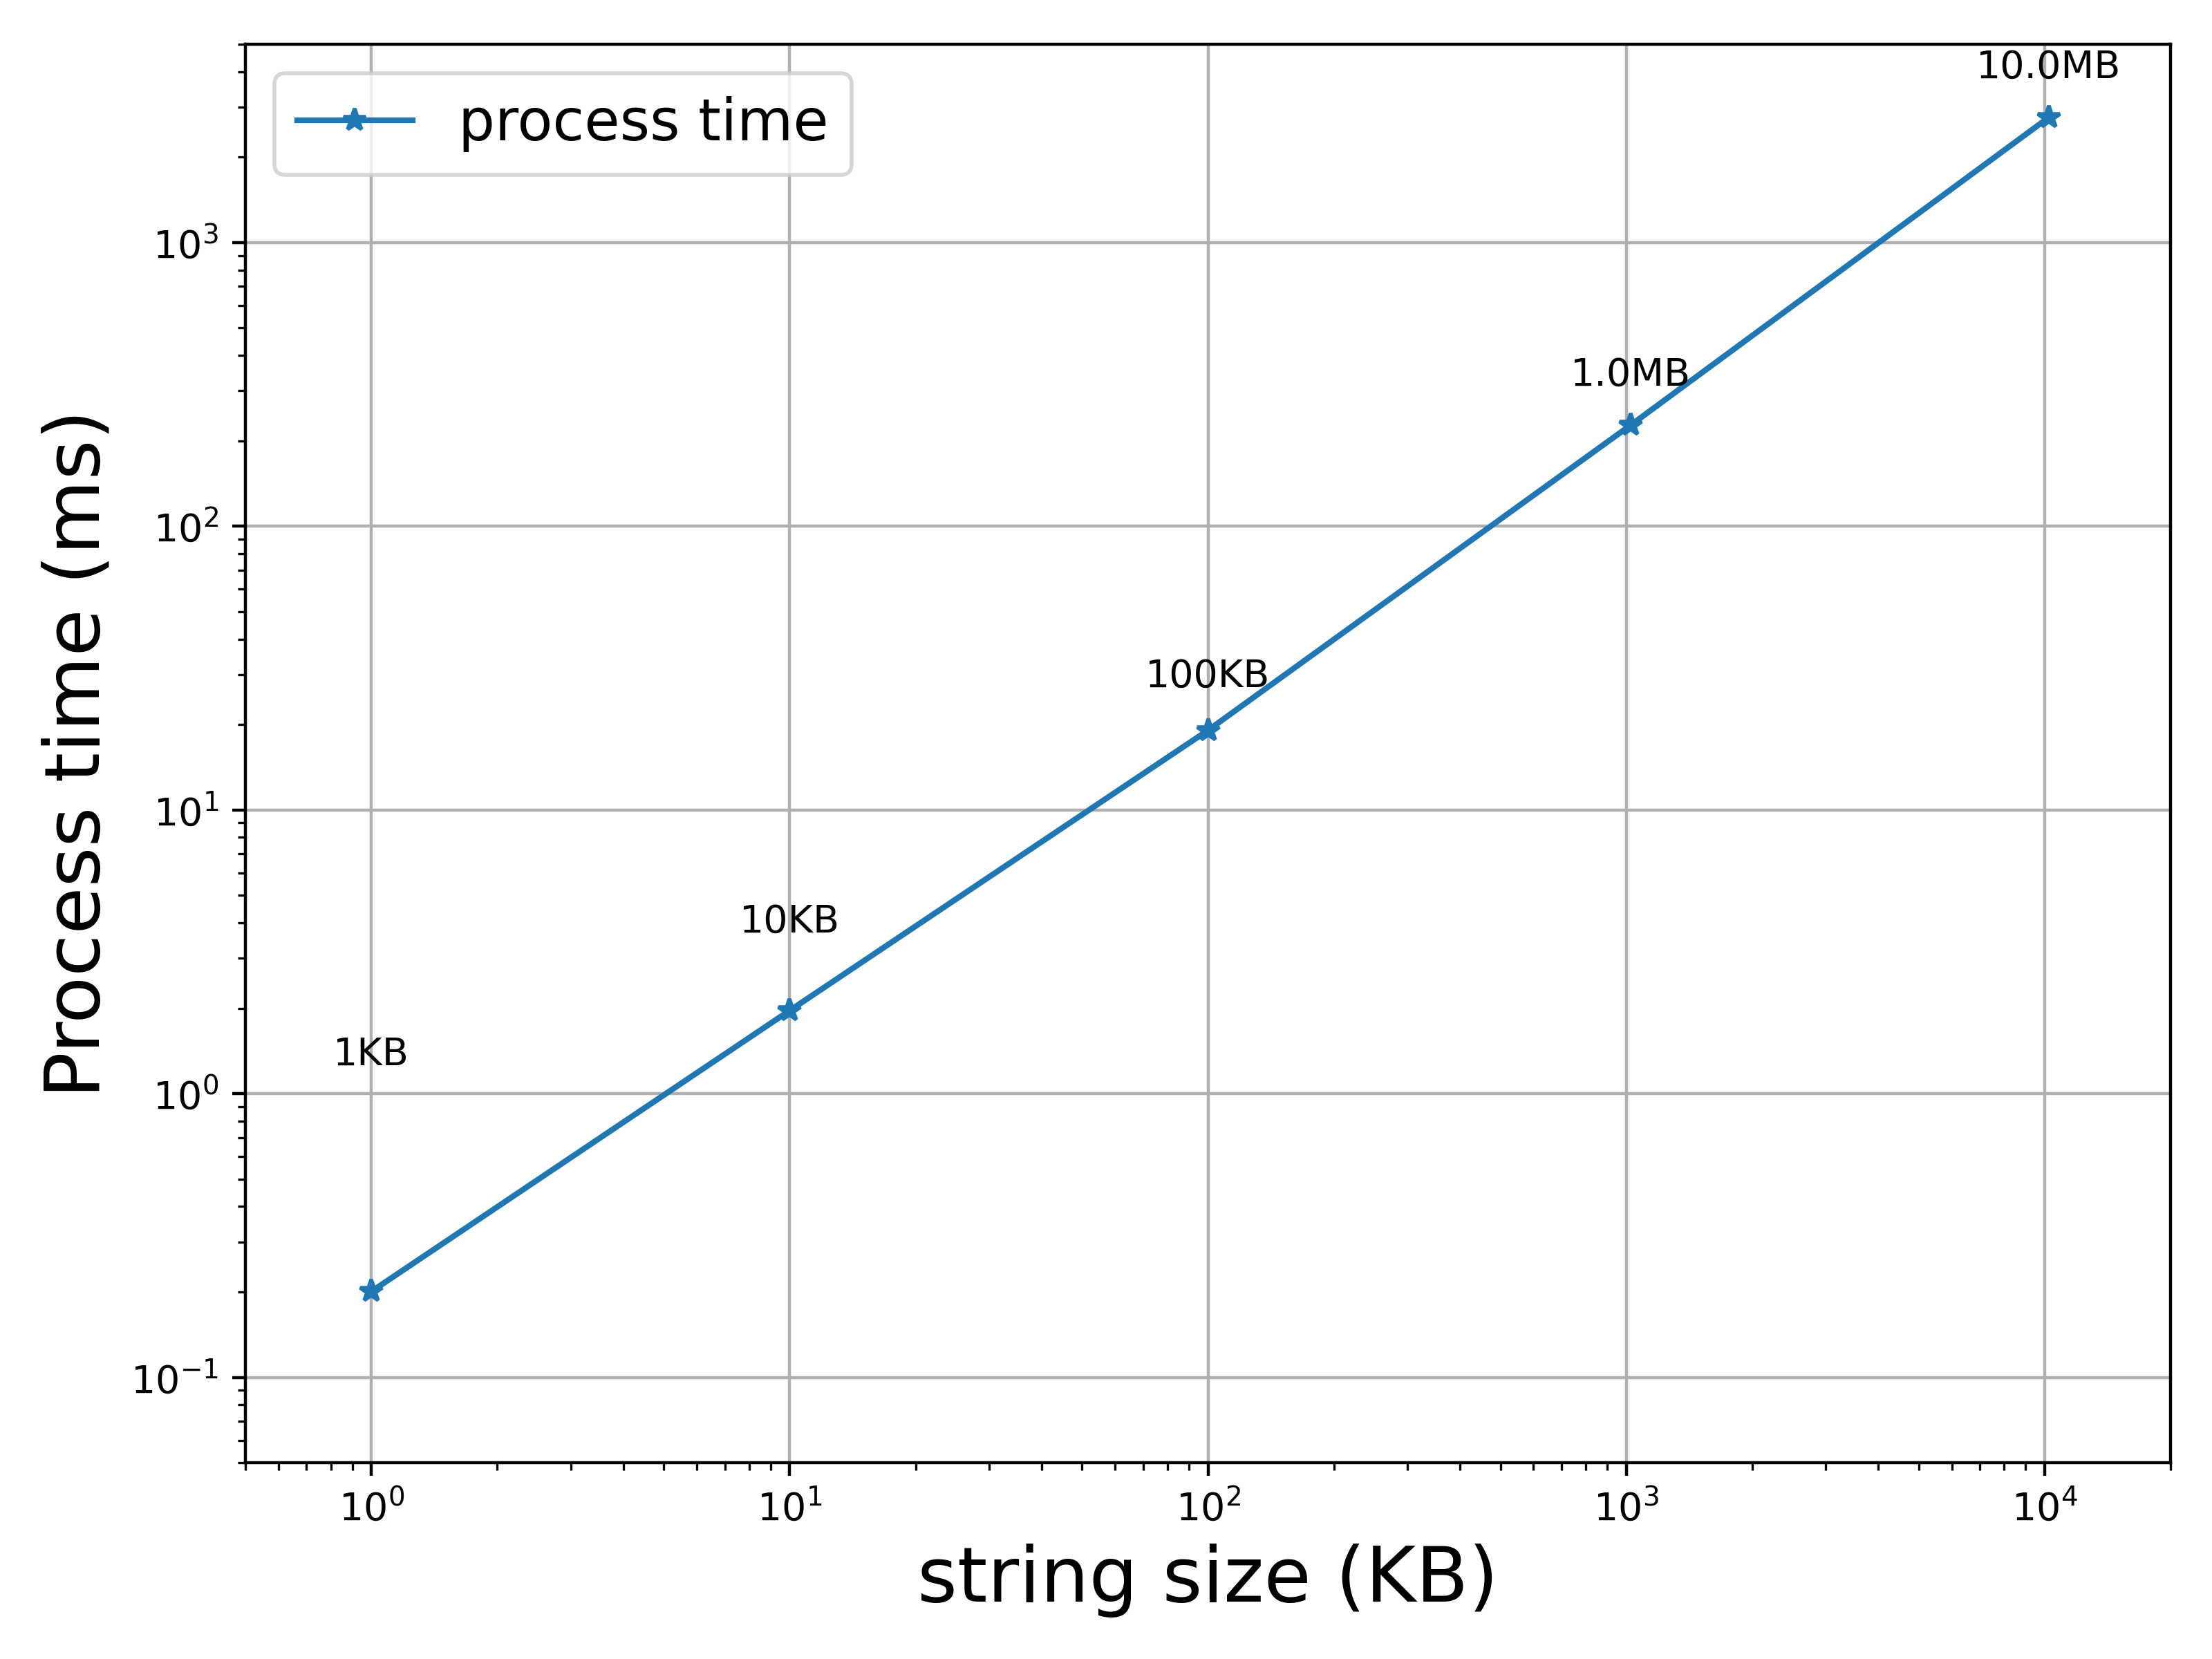
\includegraphics[width=\textwidth]{figures/tests/proportional_tests/Average_string_messages_sending_time_of_100_tests_1KB_to_10MB.png}
        \caption{} \label{fig: proportional-stringsize-a}
    \end{subfigure}
    \begin{subfigure}{0.49\textwidth}
        \centering
        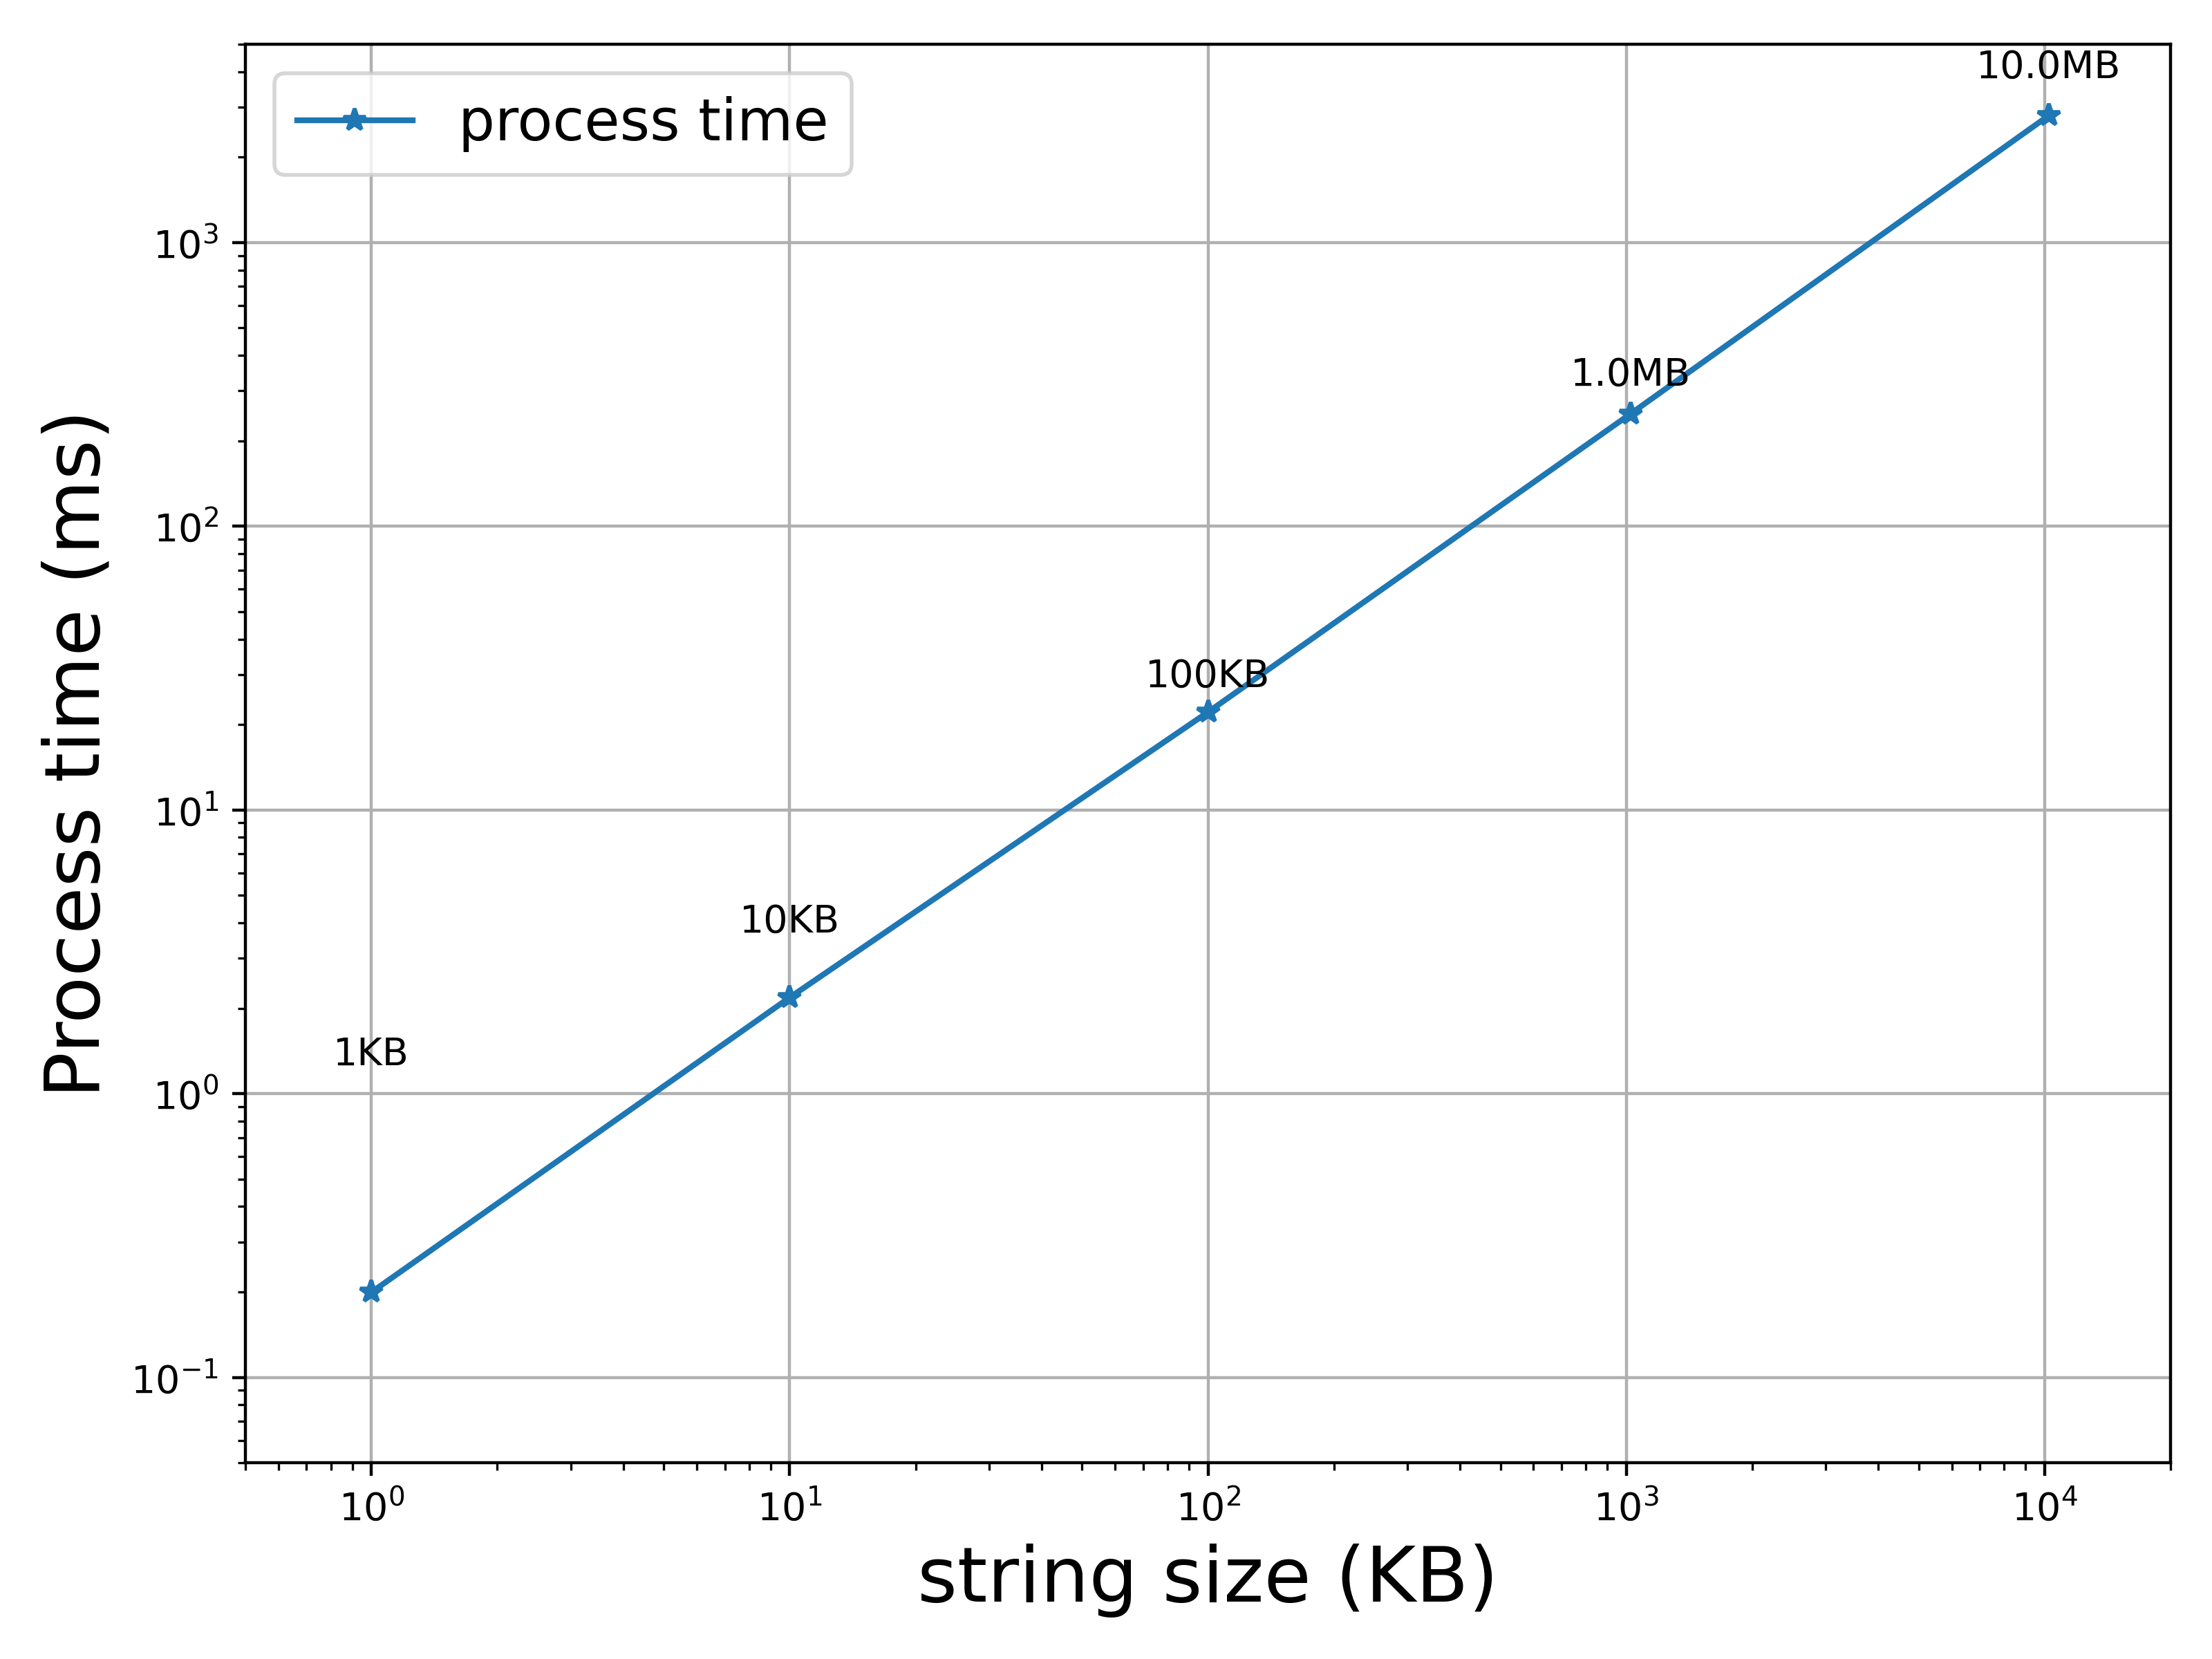
\includegraphics[width=\textwidth]{figures/tests/proportional_tests/Average_string_messages_receiving_time_of_100_tests_1KB_to_10MB.png} 
        \caption{} \label{fig: proportional-stringsize-b}
    \end{subfigure} 

    \caption{Average delay of sending and receiving a string message varied from 1KB 
    to 10MB for 100 times between 2 clients. (\subref{fig: proportional-stringsize-c}) Messages clientS sent forward, 
    (\subref{fig: proportional-stringsize-d}) response messages from clientR, 
    (\subref{fig: proportional-stringsize-a}) process time of massages sent forward 
    and (\subref{fig: proportional-stringsize-b}) process time of massages respond. 
    \label{fig: proportional-stringsize}}
\end{figure}

\subsubsection{Increasing image message length}
In addition to string, images are also frequently transported between different agents. 
However, unlike string messages, image sizes can be significantly larger, even up to over 
100MB for raw images. In addition, the agent's ID or message priority information should 
also be included in the message. Therefore, to send an image, it should be jsonified with 
the necessary information and then sent to the server. 



The tests for images are similar to those for string messages, with image size varying 
from 1KB to 100MB. Fig.\ref{fig: proportional-imagesize-a} and \ref{fig: proportional-imagesize-b} 
show the linear dependency of latency and jsonified image size. Although the transmission 
time for 1KB to 10MB messages is similar to the string test, there is a significant 
difference in process time between them. Comparing fig.\ref{fig: proportional-stringsize-c} 
with \ref{fig: proportional-imagesize-c} and fig.\ref{fig: proportional-stringsize-d} 
with \ref{fig: proportional-imagesize-d}, it is clear that the server process time for 
string messages is much higher than that for image messages. Moreover, due to the 
additional overhead of the JSON format, the network delay of string messages is 
relatively minor compared to that of image messages. 




One possible reason for the longer process time for string messages is that the server 
ust process them twice: once to split the message to extract the client ID, and again 
to recombine it for further transport. On the other hand, a jsonified image will only 
be processed once to extract the client information, and the original JSON file will 
be further transported directly.



\begin{figure}[htb]
        \centering
    \begin{subfigure}{0.49\textwidth}
        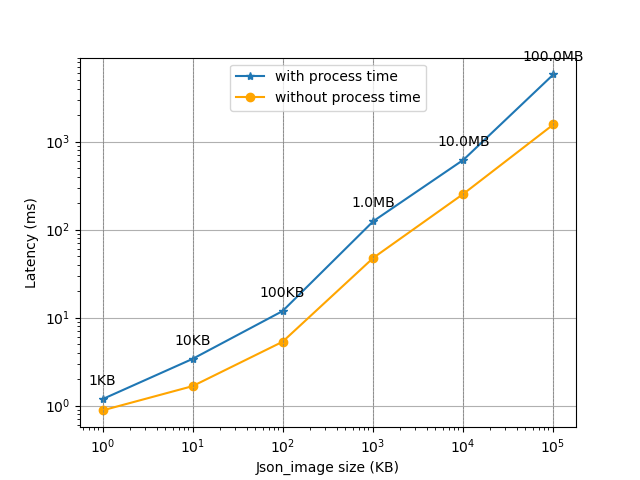
\includegraphics[width=\textwidth]{figures/tests/proportional_tests/log_Average_json_image_messages_sending_time_of_100_tests_1KB_to_100MB.png}\hfill 
        \caption{} \label{fig: proportional-imagesize-c}
    \end{subfigure}
    \begin{subfigure}{0.49\textwidth}
        \centering
        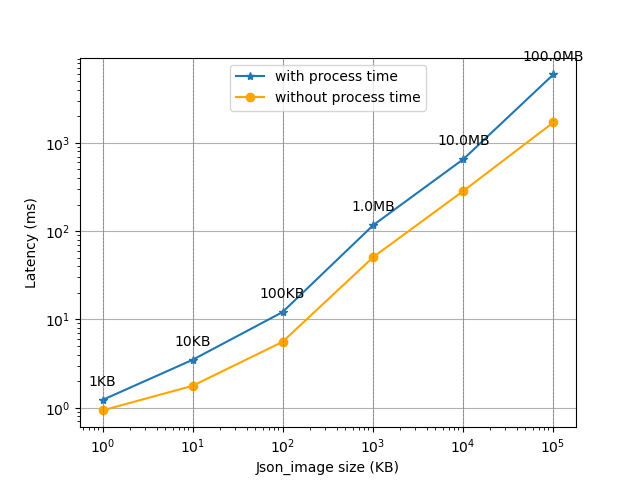
\includegraphics[width=\textwidth]{figures/tests/proportional_tests/log_Average_json_image_messages_receiving_time_of_100_tests_1KB_to_100MB.png}\hfill 
        \caption{} \label{fig: proportional-imagesize-d}
    \end{subfigure}
    \begin{subfigure}{0.49\textwidth}
        \centering
        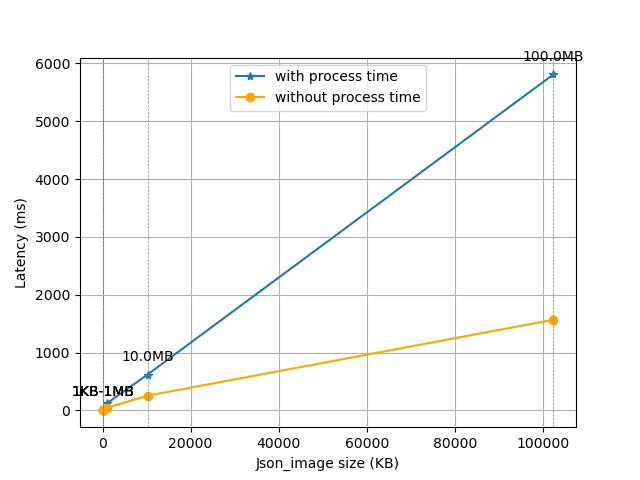
\includegraphics[width=\textwidth]{figures/tests/proportional_tests/Average_json_image_messages_sending_time_of_100_tests_1KB_to_100MB.png}\hfill 
        \caption{} \label{fig: proportional-imagesize-a}
    \end{subfigure}
    \begin{subfigure}{0.49\textwidth}
        \centering
        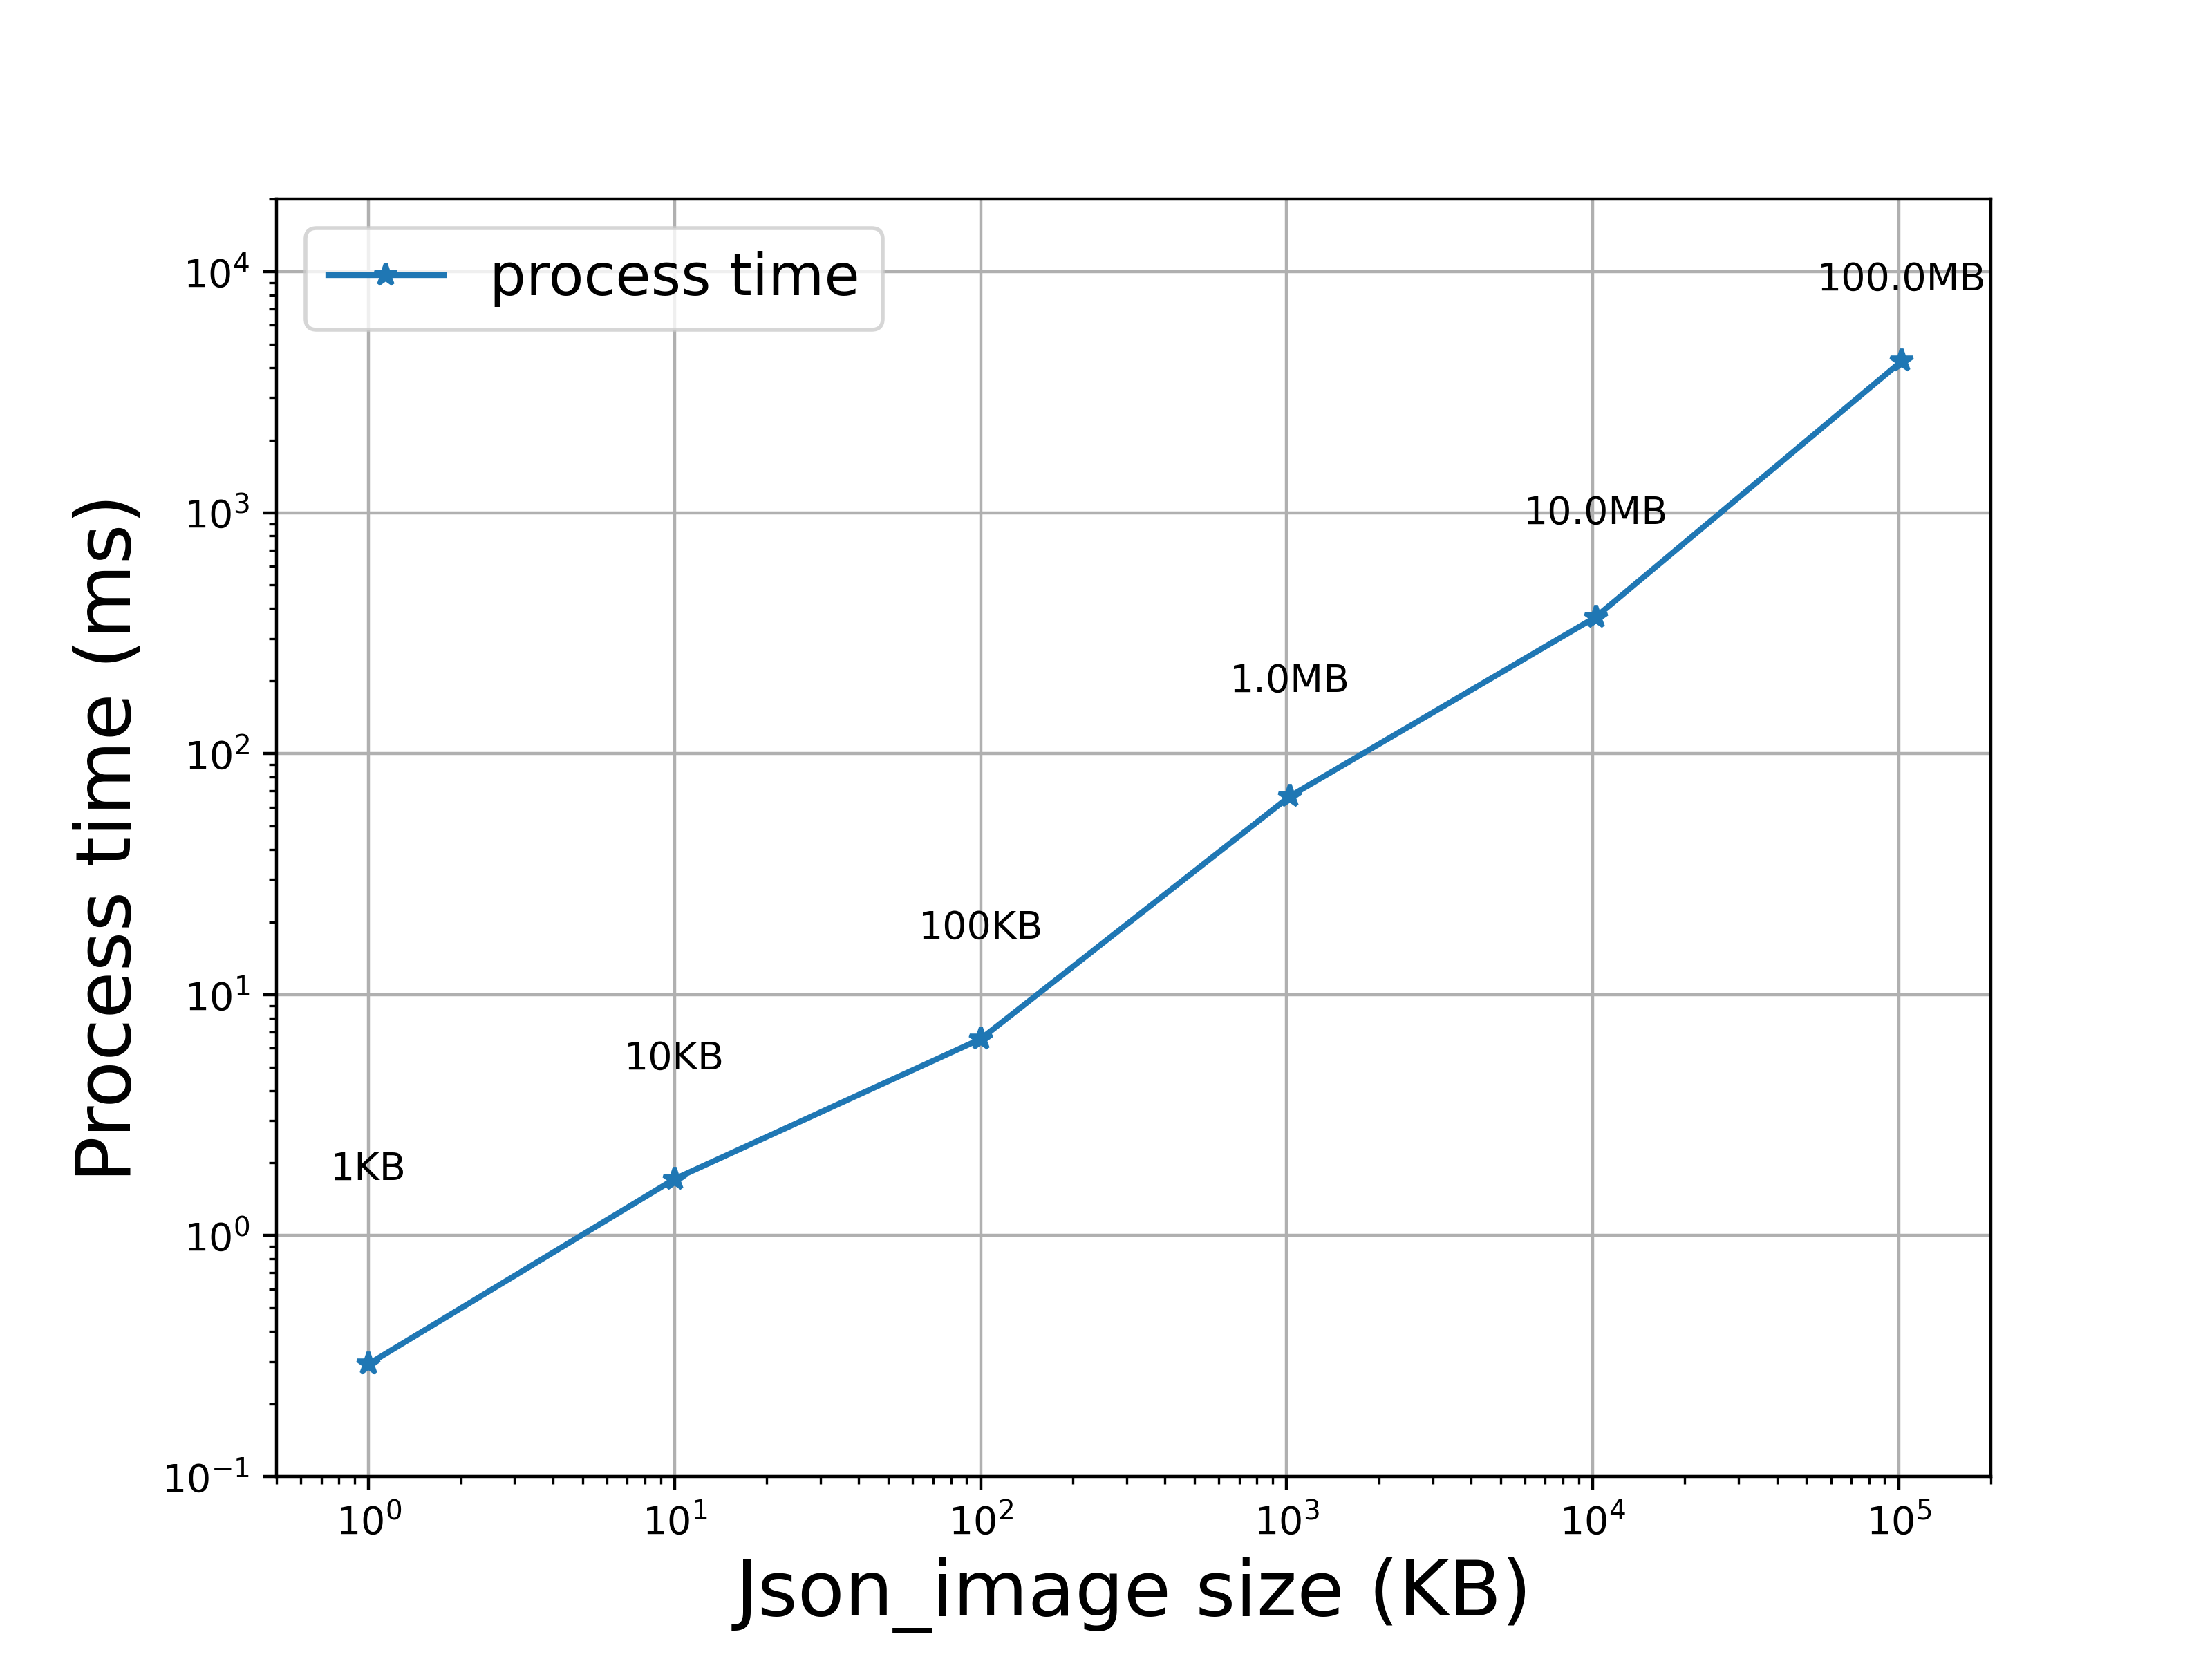
\includegraphics[width=\textwidth]{figures/tests/proportional_tests/Average_json_image_messages_receiving_time_of_100_tests_1KB_to_100MB.png}\hfill 
        \caption{} \label{fig: proportional-imagesize-b}
    \end{subfigure}

    \caption{Average delay of sending and receiving a jsonified image message varied from 1KB 
    to 100MB for 100 times between 2 clients. (\subref{fig: proportional-imagesize-c}) 
    Messages clientS sent forward in log form, 
    (\subref{fig: proportional-imagesize-d}) response messages from clientR in log form, 
    (\subref{fig: proportional-imagesize-a}) process time of messages sent forward  
    and (\subref{fig: proportional-imagesize-b}) process time of response messages from clientR. 
    \label{fig: proportional-imagesize}}
\end{figure}


\subsection{Test results of WebSocket and \gls{http}} \label{chap: Result-RestFUL_WS}
After testing the performance of the WebSocket-based communication system, it will be 
interesting to see whether the other application layer protocols with different message 
transport mechanisms will have a similar or completely different performance under the 
same conditions. As demonstrated from fig.\ref{fig: MsgConceptual}, \gls{http} is designed 
for message transport in both directions and, therefore, more comparable with WebSocket 
among the others. As a result, a \gls{http} based interface RESTful API is designed under 
a similar architecture as WebSocket and tested under the exact condition of the WebSocket 
string test in section \ref{chap: Result-Internal-string}. By comparing 
fig.\ref{fig: proportional-stringsize} with fig.\ref{fig: proportional-rest-stringsize}, 
it is evident that the processing time of string messages is higher and grows faster in 
a WebSocket server than in a RESTful API server. The difference may result in the 
prioritization and data processing mechanisms in the WebSocket server. In contrast, 
the RESTful API server is only designed with a simple message POST and GET mechanism. 
However, the data transmission time between both is more comparable. First of all, 
both of them reflect the fit of the model with the coefficient of determination close 
to one, which is namely: 


    \begin{align}
        R^{2} &= 1-\frac{RSS}{TSS}\\
        \text{Where} \nonumber\\
        RSS & = \text{sum of squared residuals} \nonumber\\
        TSS & = \text{total sum of squares}\nonumber
    \end{align}

meaning that the model fits the data well.





Secondly, the transmission time of both is similar 
for the same string message length (RESTful has slightly higher latency), with a difference 
of 0.01ms to a few milliseconds, which grows over message size. 



Therefore, WebSocket is proven more appropriate for real-time message transport, 
essential for an agent-based system.


\begin{figure}[htb]
    \begin{subfigure}[b]{0.49\textwidth}
        \centering
        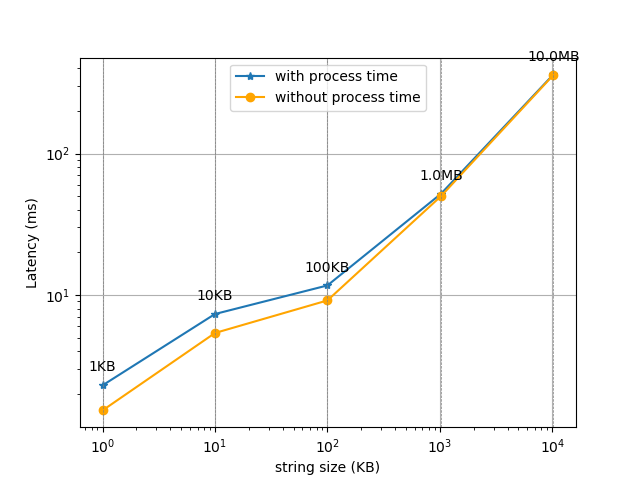
\includegraphics[width=\textwidth]{figures/tests/proportional_tests/Rest_log_Average_string_messages_sending_time_of_100_tests.png}\hfill 
        \caption{} \label{fig: proportional-rest-stringsize-c}
    \end{subfigure}
    \begin{subfigure}[b]{0.49\textwidth}
        \centering
        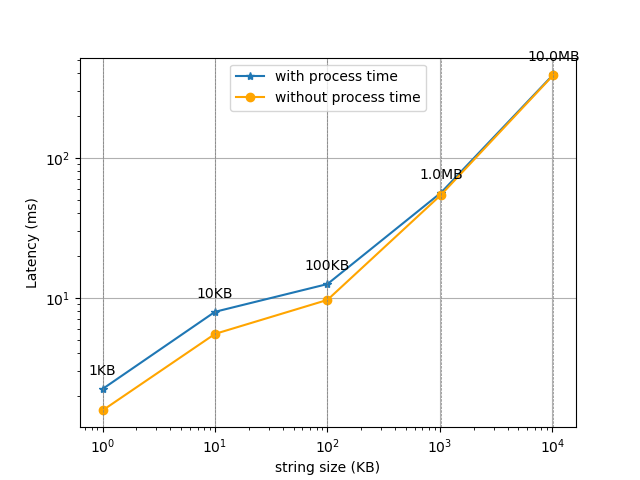
\includegraphics[width=\textwidth]{figures/tests/proportional_tests/Rest_log_Average_string_messages_receiving_time_of_100_tests.png}\hfill 
        \caption{} \label{fig: proportional-rest-stringsize-d}
    \end{subfigure}

    \begin{subfigure}[b]{0.49\textwidth}
        \centering
        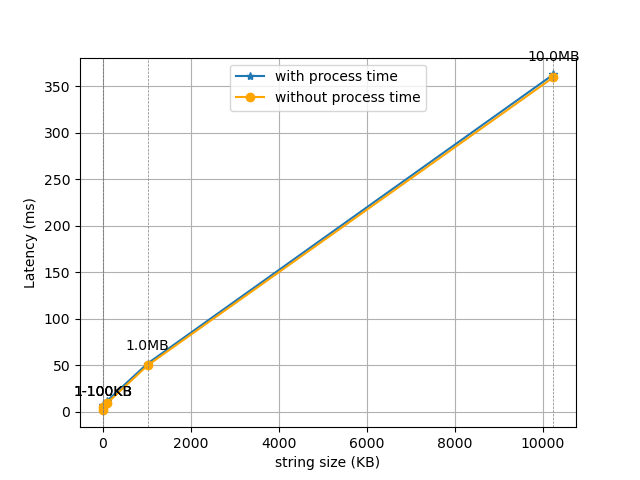
\includegraphics[width=\textwidth]{figures/tests/proportional_tests/Rest_Average_string_messages_sending_time_of_100_tests.png}\hfill 
        \caption{} \label{fig: proportional-rest-stringsize-a}
    \end{subfigure}
    \begin{subfigure}[b]{0.49\textwidth}
        \centering
        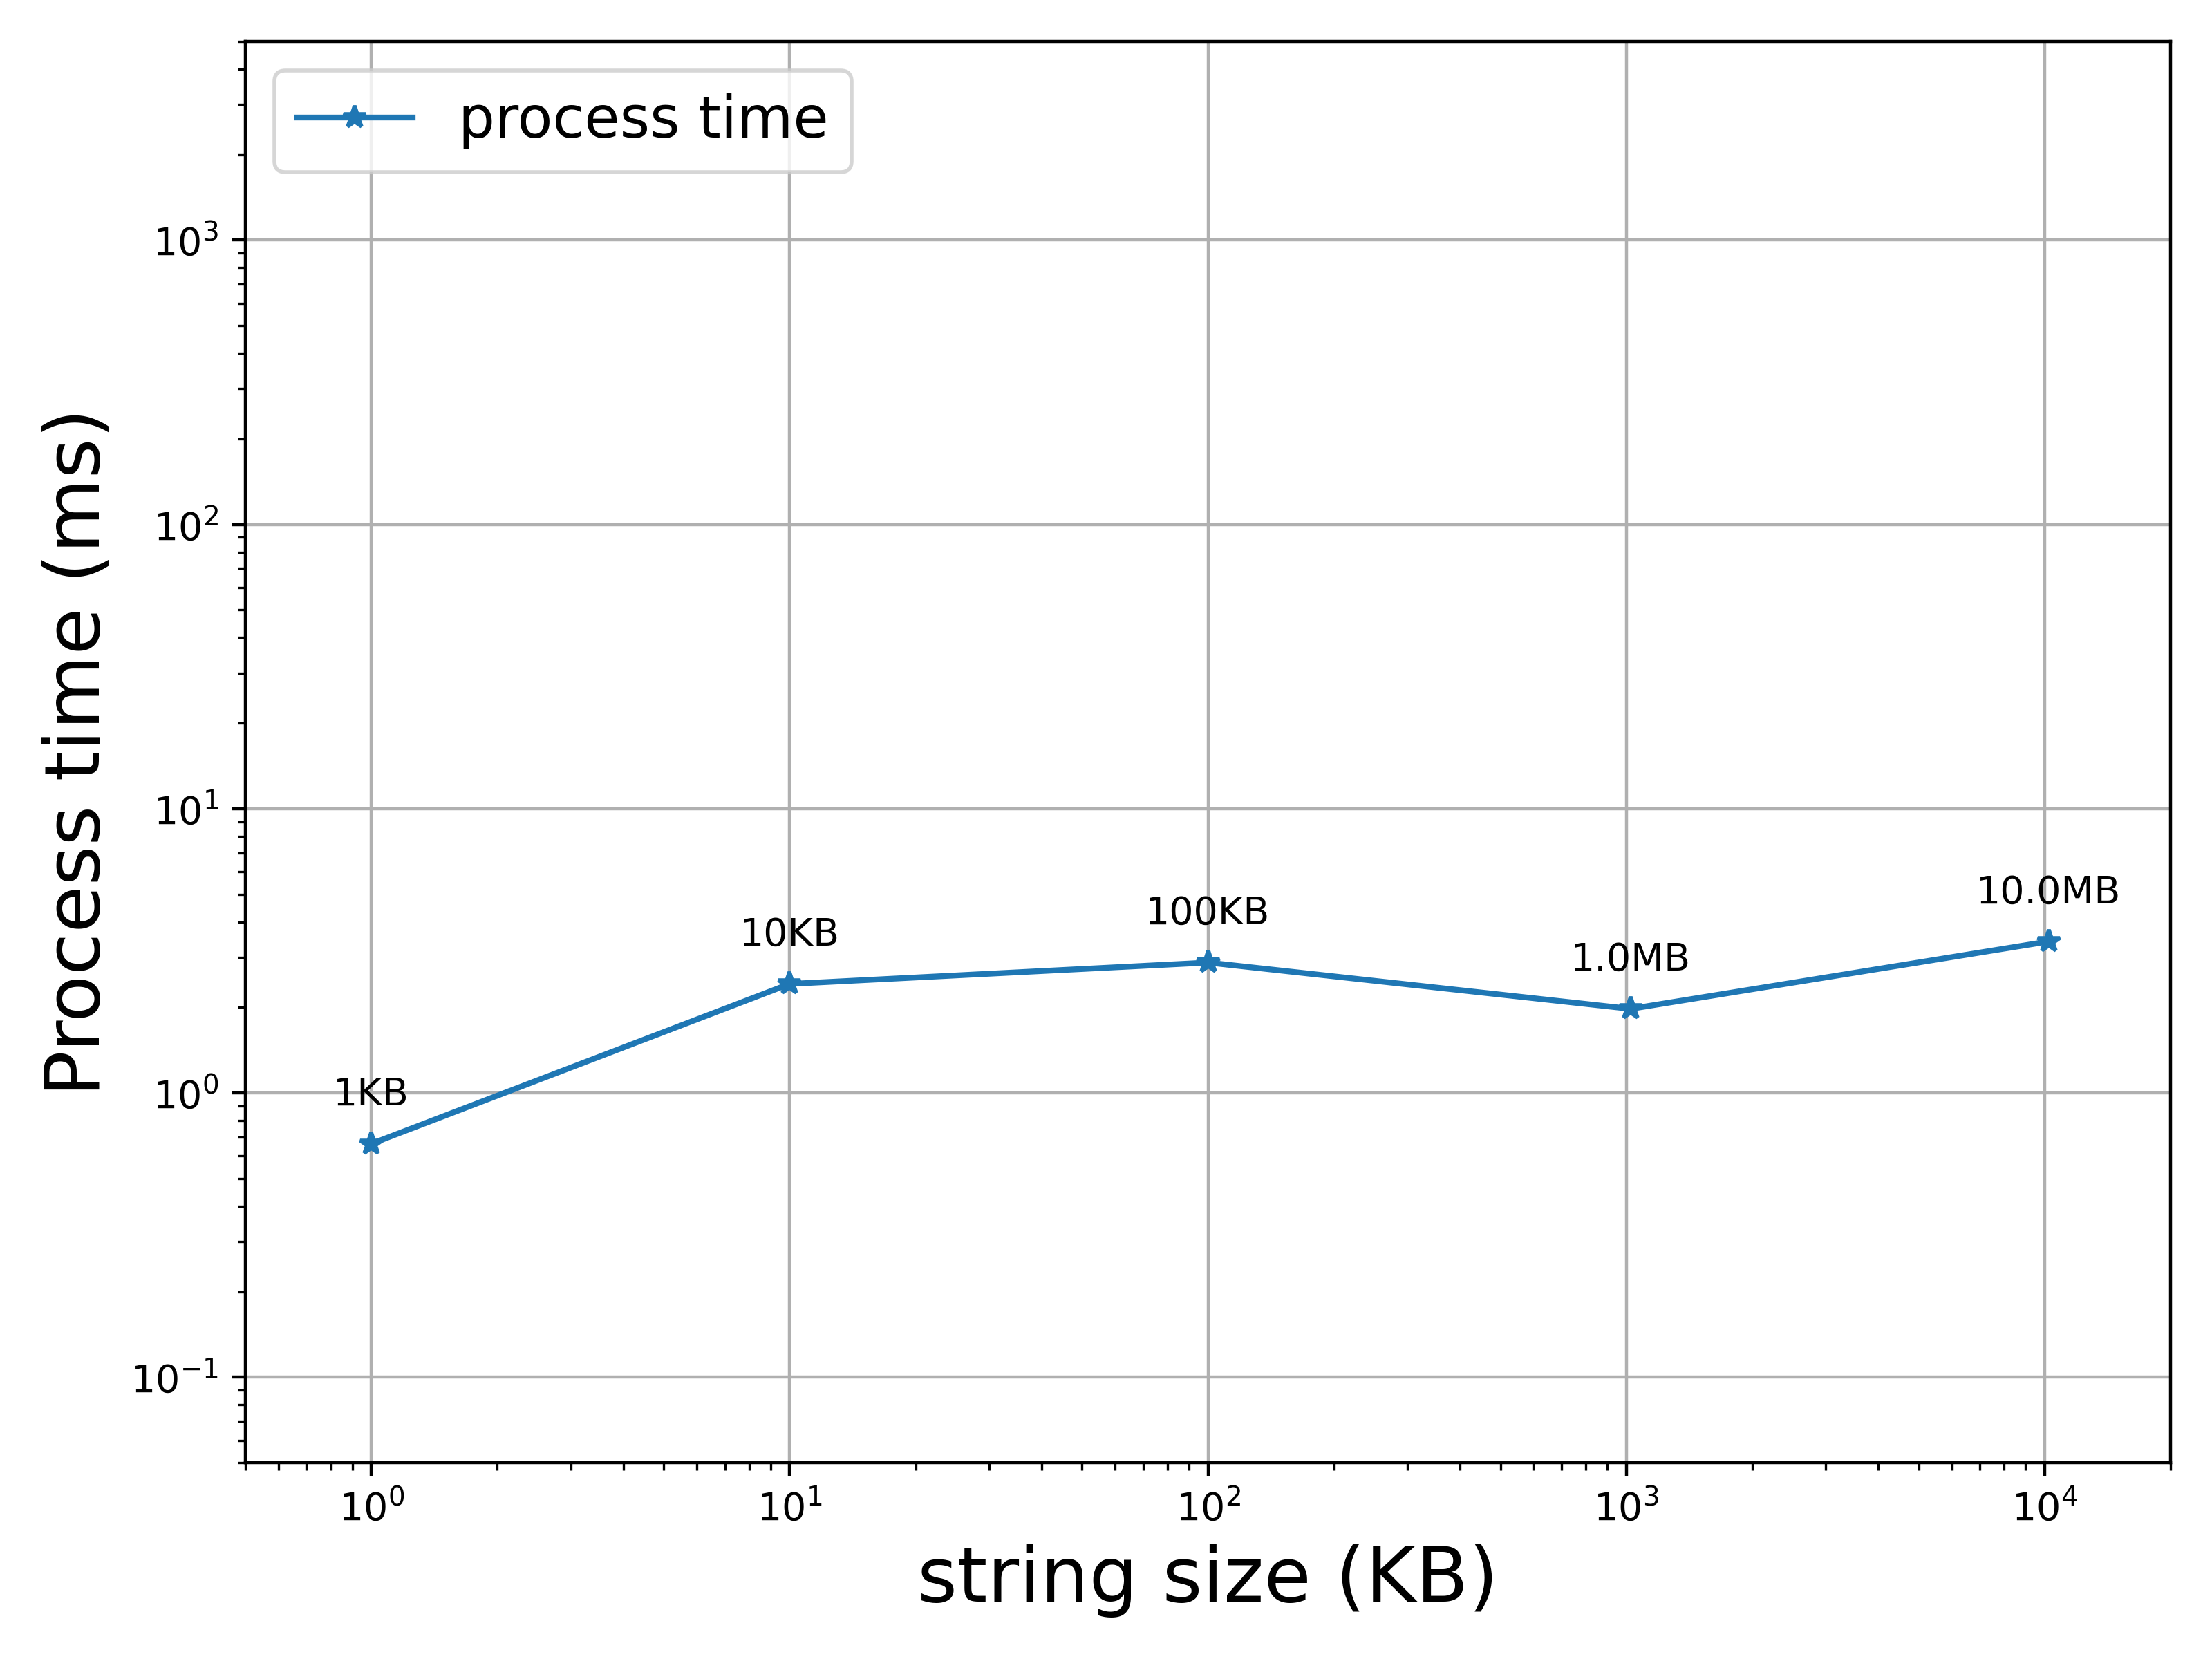
\includegraphics[width=\textwidth]{figures/tests/proportional_tests/Rest_Average_string_messages_receiving_time_of_100_tests.png}\hfill 
        \caption{} \label{fig: proportional-rest-stringsize-b}
    \end{subfigure}
    
    \caption{RESTful API: Average delay of sending and receiving a string message varied from 1KB 
    to 10MB for 100 times between 2 clients. (\subref{fig: proportional-rest-stringsize-c}) 
    Messages clientS sent forward, 
    (\subref{fig: proportional-rest-stringsize-d}) response messages from clientR, 
    (\subref{fig: proportional-rest-stringsize-a}) process time of messages sent forward 
    and (\subref{fig: proportional-rest-stringsize-b}) process time of messages respond. 
    \label{fig: proportional-rest-stringsize}}
\end{figure}





\subsection{Test results of message prioritization in a WebSocket server with various 
performance testing} \label{chap: Result-priority}
In an agent communication system, the server that serves as a \gls{ca} should not only 
focus on speed, robustness, reliability, and application size, but also have additional 
functionalities beyond pure message transport. Table \ref{tab:designPatterns} lists the 
essential design requirements of a \gls{ca}, which should include a communication interface 
capable of processing various messages with different data types such as jsonified images, 
handling a large number of agent connections, and prioritizing incoming messages. 
In the following sections, we will test and discuss the server's performance in 
handling message prioritization.

\subsubsection{Measurgin method}
In order to verify the prioritization mechanism of the server, a delay of 1s should be 
added to the non-prioritized message processing. In the test, two kinds of messages are 
sent concurrently to the server: the normal and the critical messages. If multiple 
messages with different priority levels enter the server simultaneously, the critical 
messages should be processed first. The add-up of delay also reflects real-world scenarios. 
Suppose a critical message representing an emergent stop or a task with higher priority 
in production comes in. In that case, every other process in the server should wait until 
the critical message is sent. 

\subsubsection{String message priority test}
The first string priority test is performed for ten clients. The following 
fig.\ref{fig: priority-10clients-a} and \ref{fig: priority-10clients-b} show the 
mean \gls{rtt} that a non-prioritized and prioritized message is being sent forward and 
back separately for 100 times.
Fig.\ref{fig: priority-10clients-a} shows the mean RTT for client1 to client10 in both 
directions, which ranges from 0.63ms to 1.09ms. These figures meet the near real-time 
requirement for the production process. On the other hand, fig.\ref{fig: priority-10clients-b} 
illustrates the timing differences between normal messages as a group and critical messages 
as a control group. In this test, all clients except client10 delivered normal messages. 
The server paused other processes for 1s and handled the critical message immediately 
whenever a critical message from client10 arrived. The mean RTT for client10 was less 
than 1ms, while clients such as client1 through client5 and client9 experienced 
significantly higher RTTs, sometimes reaching several hundred milliseconds. This 
verified the assumption of message prioritization. It is worth mentioning that the 
asyncio package used in the WebSocket server design is concurrent. Therefore, each 
client is executed one after another, rather than in parallel processing. As a result, 
some messages may never be paused if the clients' execution process is not synchronized 
and coordinated explicitly.

\begin{sidewaysfigure}[htb]
    \centering
    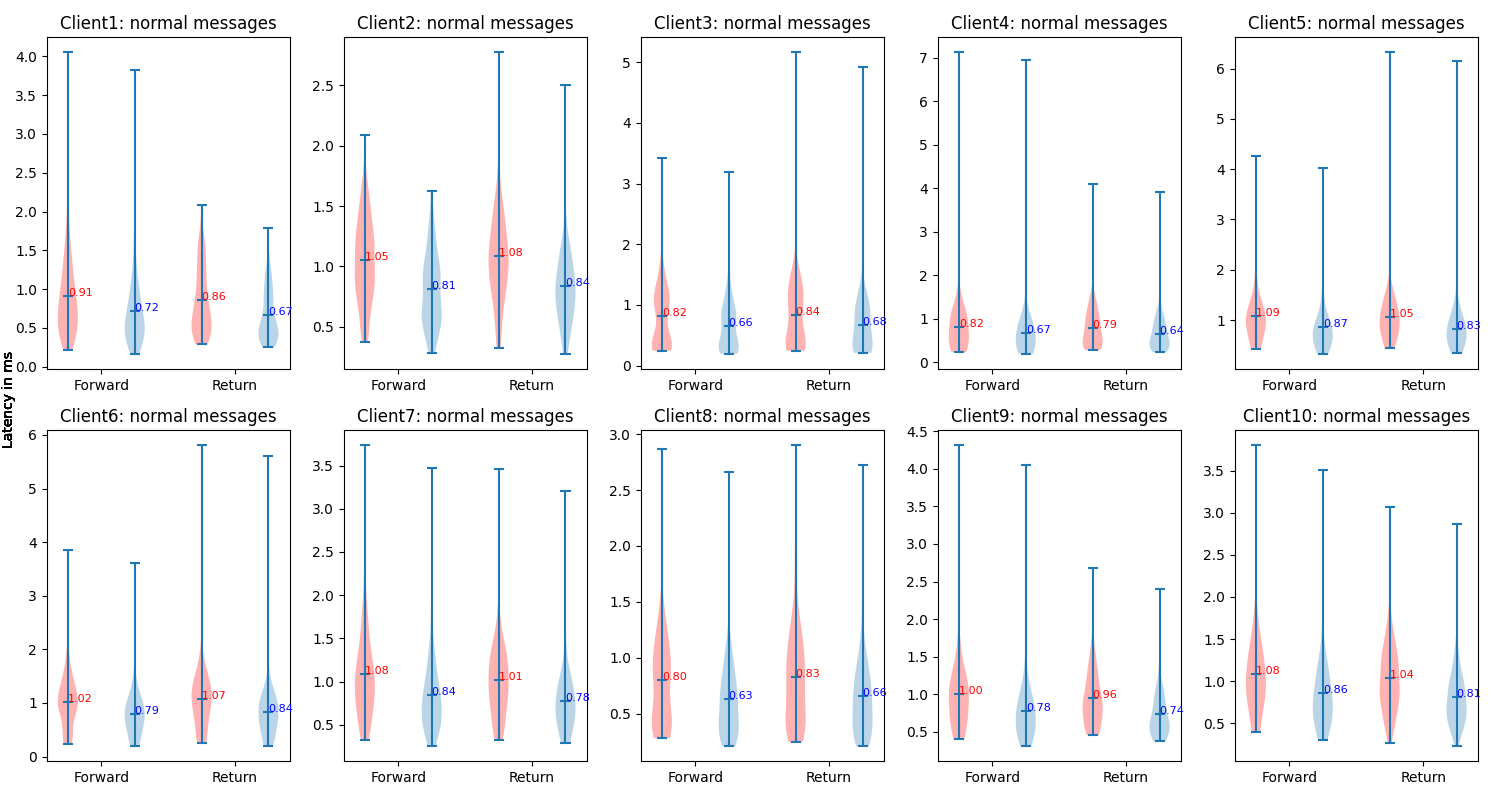
\includegraphics[width=\textheight]{figures/tests/priority_tests/violin_10clients_string_non_priority.png}\hfill 
    \caption{Tests for mean \gls{rtt} of forward and return non-prioritized string messages between 10 clients 
    and clientR for 100 times. The blue violin represents the average data transmission time and the red violin 
    respresent mean \gls{rtt}.} \label{fig: priority-10clients-a}
\end{sidewaysfigure}
\begin{sidewaysfigure}[htb]
    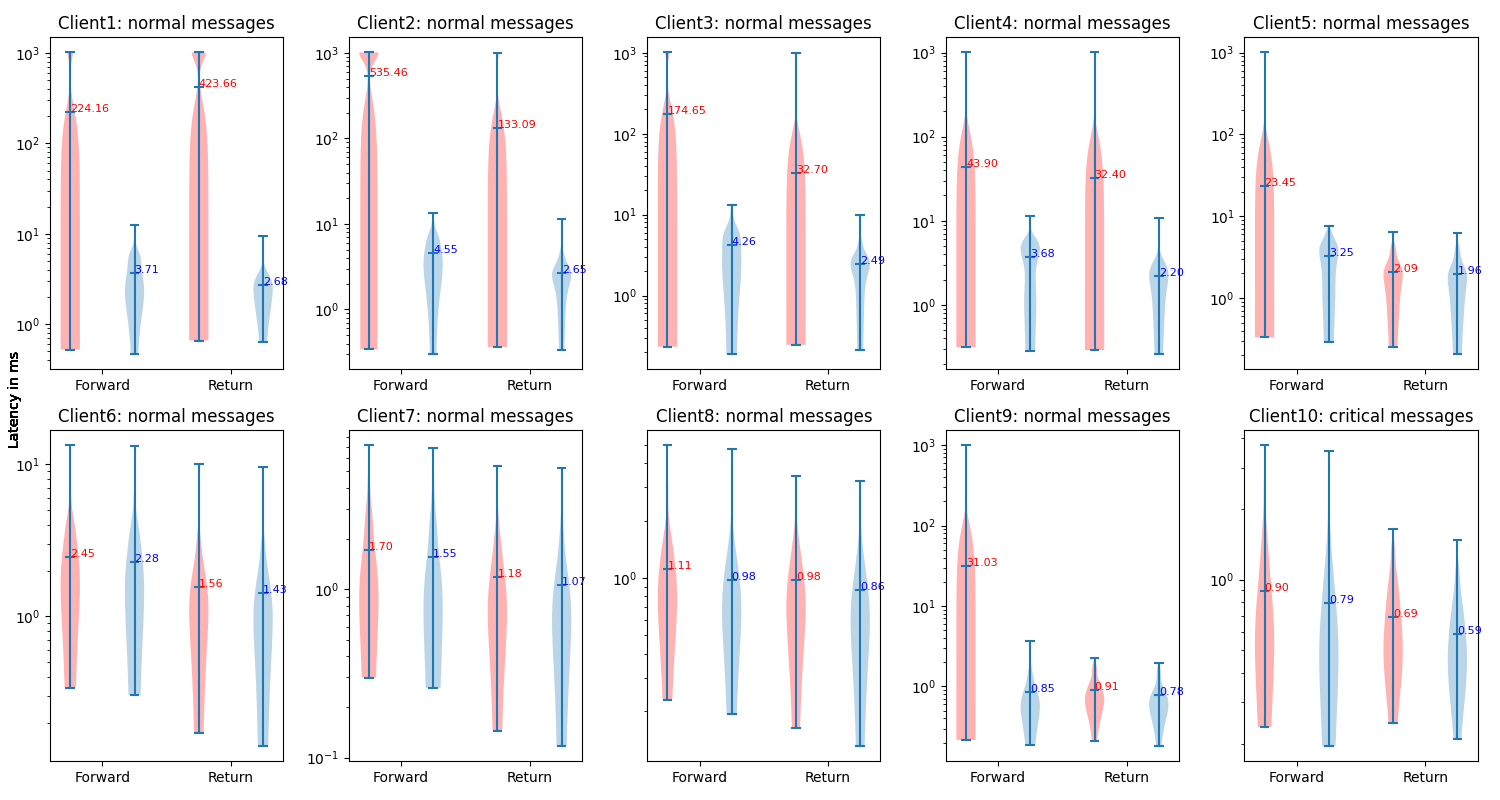
\includegraphics[width=\textheight]{figures/tests/priority_tests/log_violin_10clients_string_priority.png}\hfill 
    \caption{Tests for mean \gls{rtt} of forward and return prioritized string messages between 10 clients 
    and clientR for 100 times. The blue violin represents the average data transmission time and the red violin 
    respresent mean \gls{rtt}.} \label{fig: priority-10clients-b}
\end{sidewaysfigure}





As part of our testing process, priority tests are performed for ten clients across 
various scales, with the number of clients varying from 2 to 10 to 50. The test results 
of two clients can be found in \ref{chap: append-string-priority} fig.\ref{fig: priority-2clients-string}, 
and those for fifty clients in fig.\ref{fig: priority-50clients-string-a} to 
\ref{fig: priority-50clients-string-e}.  The results of the string message priority 
test with two clients clearly show that client 1 sent messages with lower priority, 
resulting in significantly higher delays than client 2 in both directions. In the test 
with fifty clients, the results were similar to those of the ten-client test. Only the 
last client sent a critical message, while the other 49 sent normal messages. As a 
result, some clients were affected by the mechanism, causing significant delays, while 
client 50 always had the smallest round-trip time.

\subsubsection{Image message priority test}
The same tests are also done for image message transport. Slightly different from string 
messages, the prioritization jsonified image file (image size: 33.4KB) will be performed 
after deserialization. In the image priority test, client1 to client10 will send an image 
to clientR and receive a string message as a response. In actual production, a confirm 
string message will be sent back if the clientR successfully receives the image message. 
Therefore, this test better reflects the time difference between different message types 
in the actual production process since the actual string length will be much smaller than 
the image length. As shown in fig.\ref{fig: priority-10clients-c}, it proves that the data 
transmission time or the server process time of an image message 
will be higher than that of a string message.


\begin{sidewaysfigure}[htb]
    \centering
    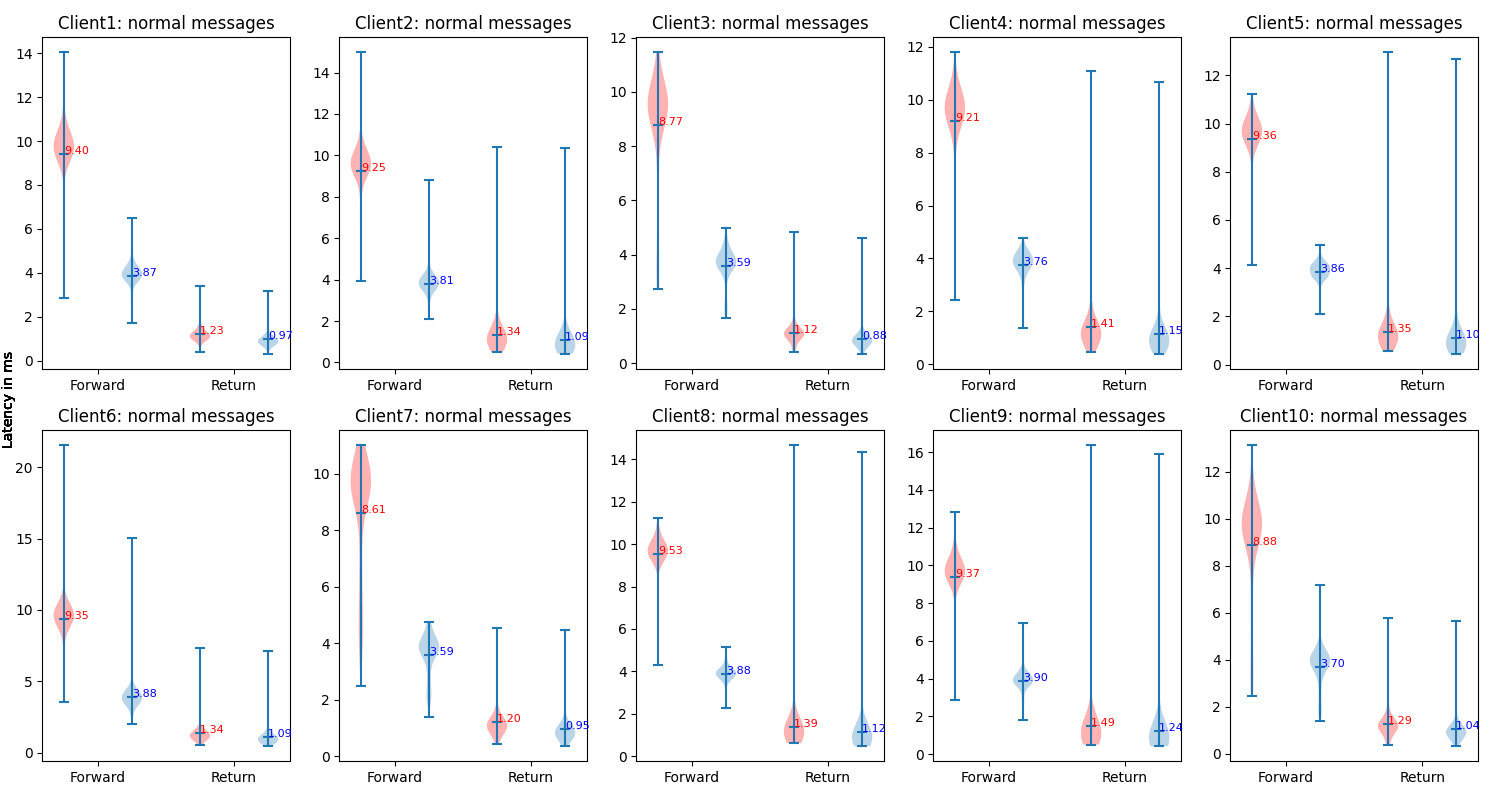
\includegraphics[width=\textheight]{figures/tests/priority_tests/violin_10clients_image_non_priority.png}\hfill 
    \caption{Tests for mean \gls{rtt} of non-prioritized forward image messages and return string messages between 10 clients 
    and clientR for 100 times. The blue violin represents the average data transmission time and the red violin 
    respresent mean \gls{rtt}.} \label{fig: priority-10clients-c}
\end{sidewaysfigure}


Another test (fig.\ref{fig: priority-10clients-d}) should be similar to the string message priority test In the upcoming test (fig.\ref{fig: priority-10clients-d}), 2, 10, and 50 clients will send images and receive string messages as a response from clientR. All clients, except client10, will send normal image messages while client10 will send a critical one to the clientR. The prioritization mechanism will be triggered for all image messages and a part of the response string messages. Notably, the prioritized string messages' latency in this test is similar to the previous test results (fig.\ref{fig: priority-10clients-b}). 

This can be attributed to the fact that larger file sizes require longer transport and 
processing times. As the image message length increases, more data bytes need to be 
processed simultaneously, resulting in more message queuing and prioritization in the 
server. A similar conclusion can be drawn from the tests conducted for 2 and 50 clients 
in fig.\ref{fig: priority-2clients-image} to fig.\ref{fig: priority-50clients-image-e} 
in \ref{chap: append-image-priority}., 
with 2, 10 and 50 clients sending images and receiving string messages as a response 
from clientR. All client1 to client9 send a normal image message, and meanwhile client10 
sends a critical one to the clientR. In the test, all image messages and only a part of 
the response string messages being sent trigger the prioritization mechanism. In this, 
the latency for the prioritized string messages is very similar to previous test results.
The reason might be that the larger the file size, the longer the transport 
and processing time will be required. The more significant message length of images 
results in more data bytes that need to be processed simultaneously, which involves 
more message queuing and prioritization in the server. The same conclusion can also be 
made for the tests for 2 and 50 clients in \ref{chap: append-image-priority} 
fig.\ref{fig: priority-2clients-image} to \ref{fig: priority-50clients-image-e}.


\begin{sidewaysfigure}[htb]
    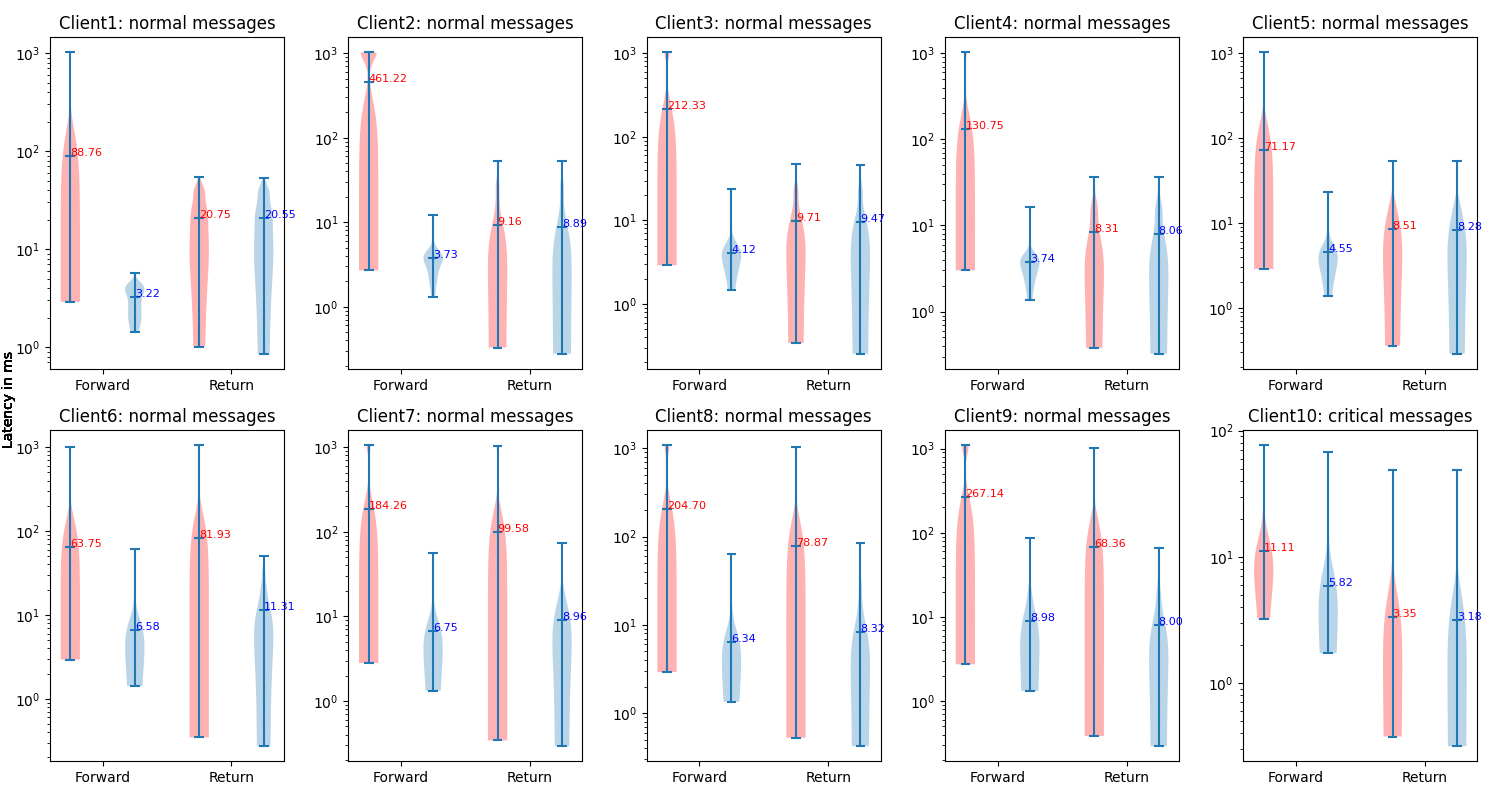
\includegraphics[width=\textheight]{figures/tests/priority_tests/log_violin_10clients_image_priority.png}\hfill 
    \caption{Tests for mean \gls{rtt} of prioritized forward image messages and return string messages between 10 clients 
    and clientR for 100 times. The blue violin represents the average data transmission time and the red violin 
    respresent mean \gls{rtt}.} \label{fig: priority-10clients-d}
\end{sidewaysfigure}


\subsection{Diagrams of \gls{mas} architecture under two use cases and 
test results of BMW use case}\label{chap: Result-Internal-Usecase}

As mentioned earlier in the form of pseudocode in Section \ref{chap: Meth-WS-MAS}, 
the architecture of the \gls{mas} is designed to cater to all use cases. In the code, 
a complete workflow is designed for a standard production process in the real world, 
from agent allocation to sequenced-based agent communication. To gain a better 
understanding of the workflow of both use cases, two diagrams are provided: 
fig.\ref{fig: sequence-diagram} shows a general workflow that can be applied to all
use cases, and fig.\ref{fig: Flowchart-usecase} shows the actual workflow of the 
two use cases.


In the general use case diagram (fig.\ref{fig: sequence-diagram}), the 
design for the \gls{mas} should be identical for all use cases except for 
the availability check and primitive execution parts (production processes) in the loop. 
The detailed program execution sequence is already described in 
section \ref{chap: Meth-WS-MAS}. Something worth noting here is that the sequence 
of the production processes in the loop should be relevant to use cases, namely the 
customer requirements. That means the sequence for task execution in the test should 
be more complex. Rather than a simple round trip between three agents, sometimes the 
Transport agent can receive orders from the Storage agent and send orders to the Storage 
agent again to save time from the slow restocking of supermarket cell. However, 
the workflow in fig.\ref{fig: Flowchart-usecase} may be the best route in actual 
production based on its simplicity of agent communication design.  

\begin{figure}[htb]
    \centering
    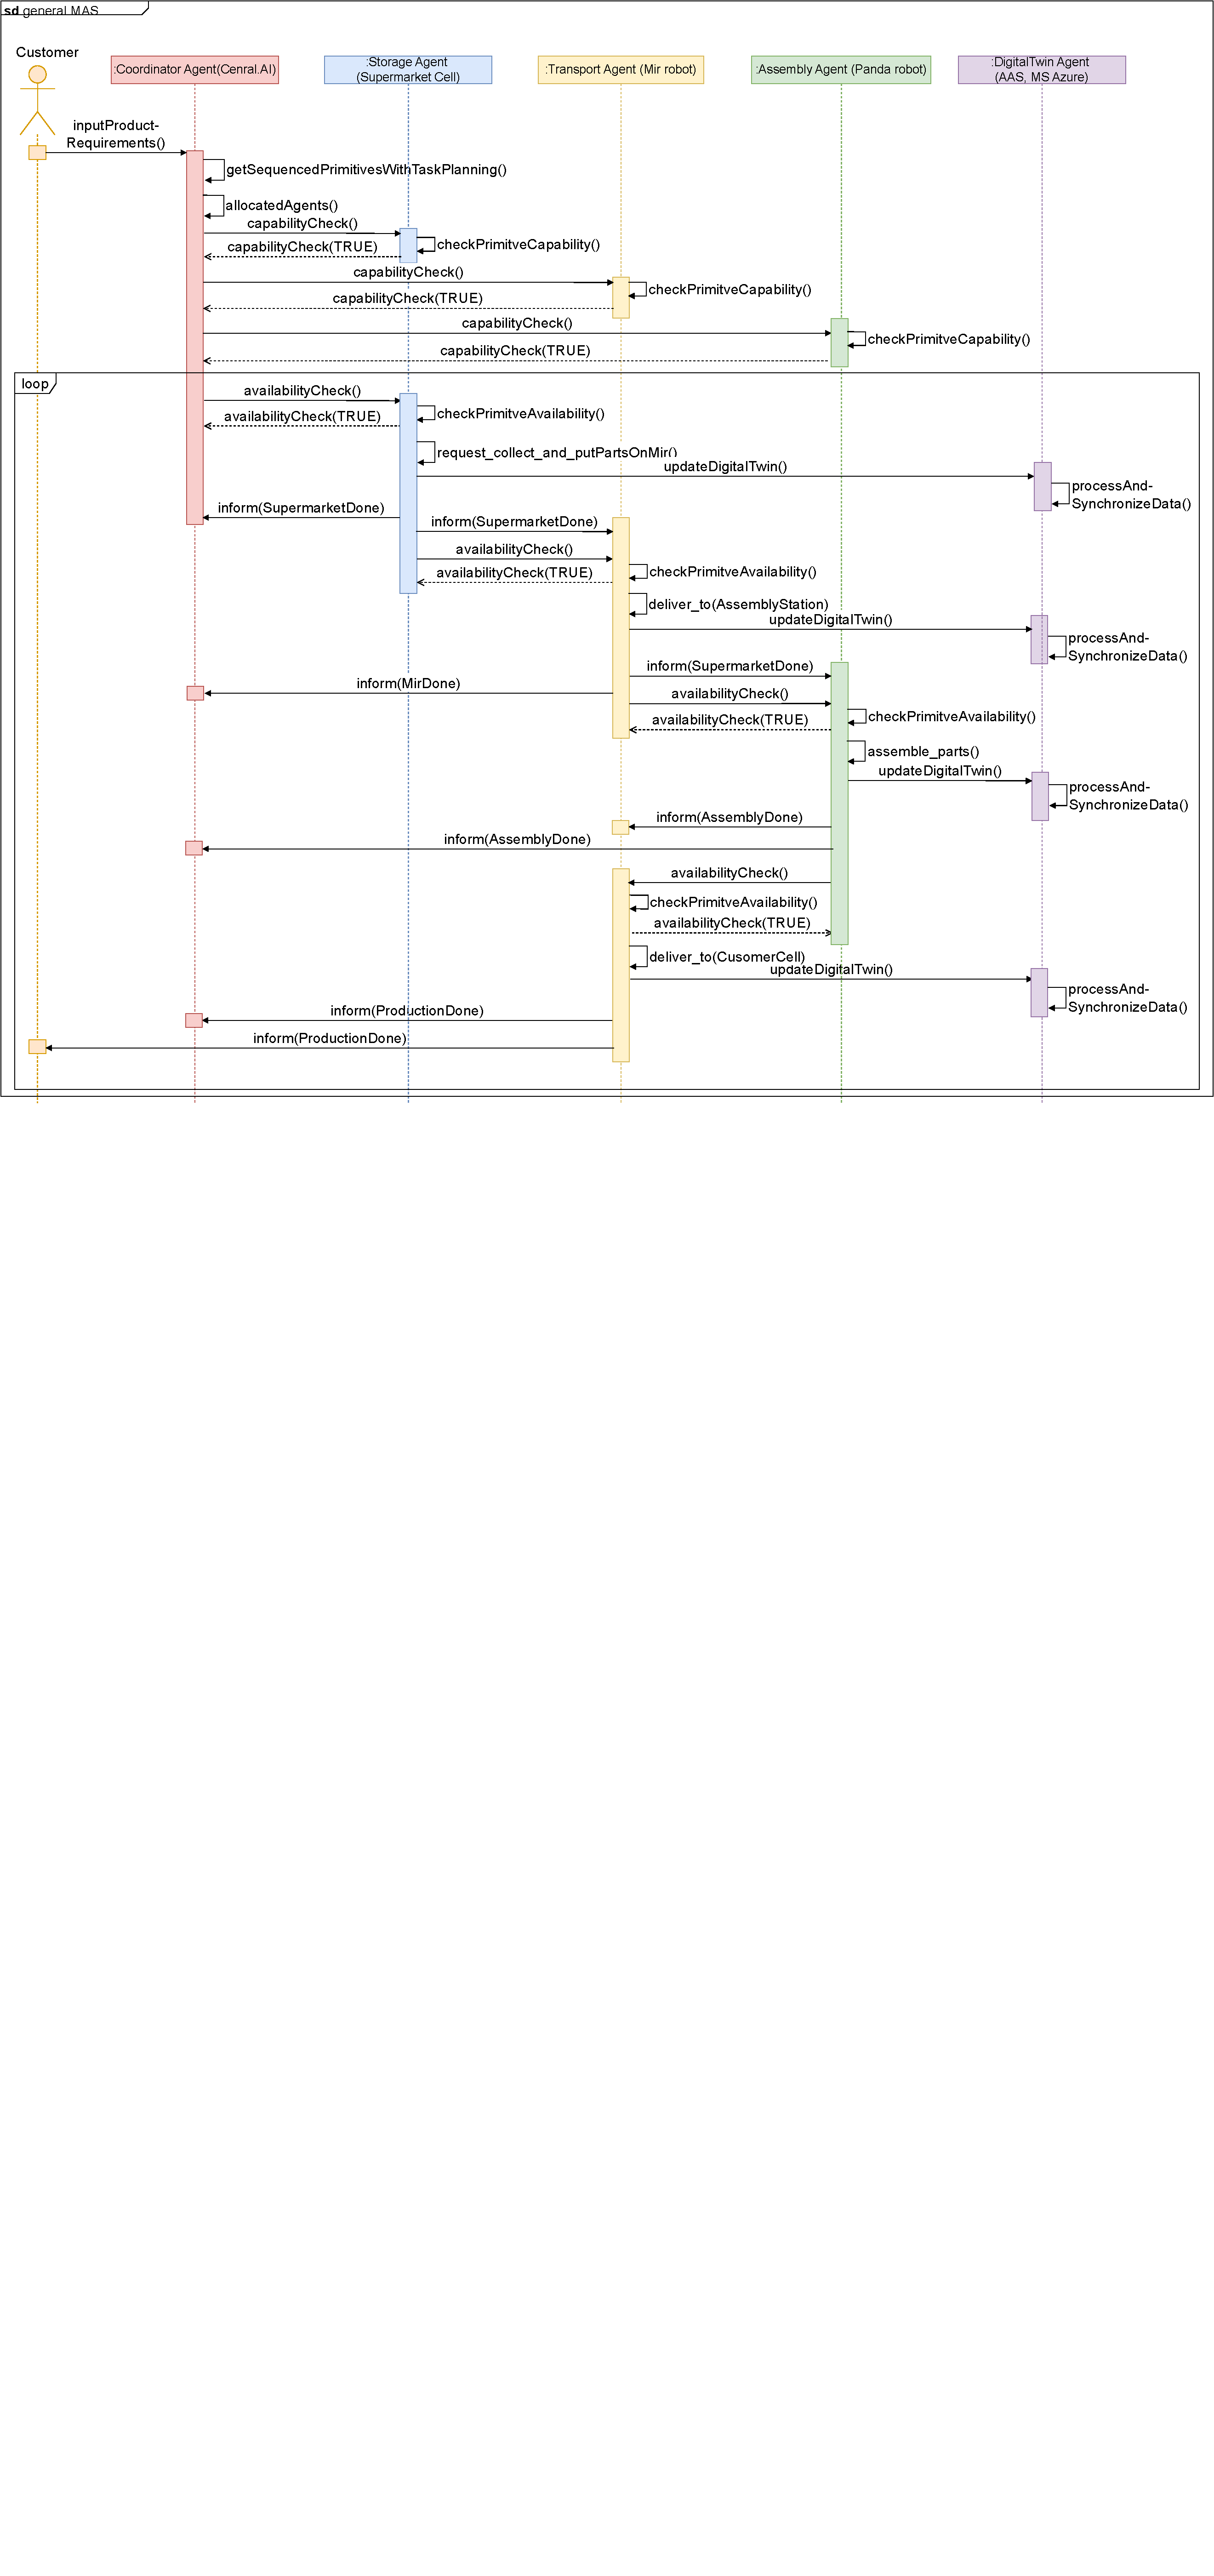
\includegraphics[width=\textwidth]{figures/tests/usecase/SequenceUsecases.pdf}\hfill 
    \caption{\gls{uml} general use case diagram of the \gls{mas} architecture.} 
    \label{fig: sequence-diagram}
\end{figure}


\begin{figure}[htb]
    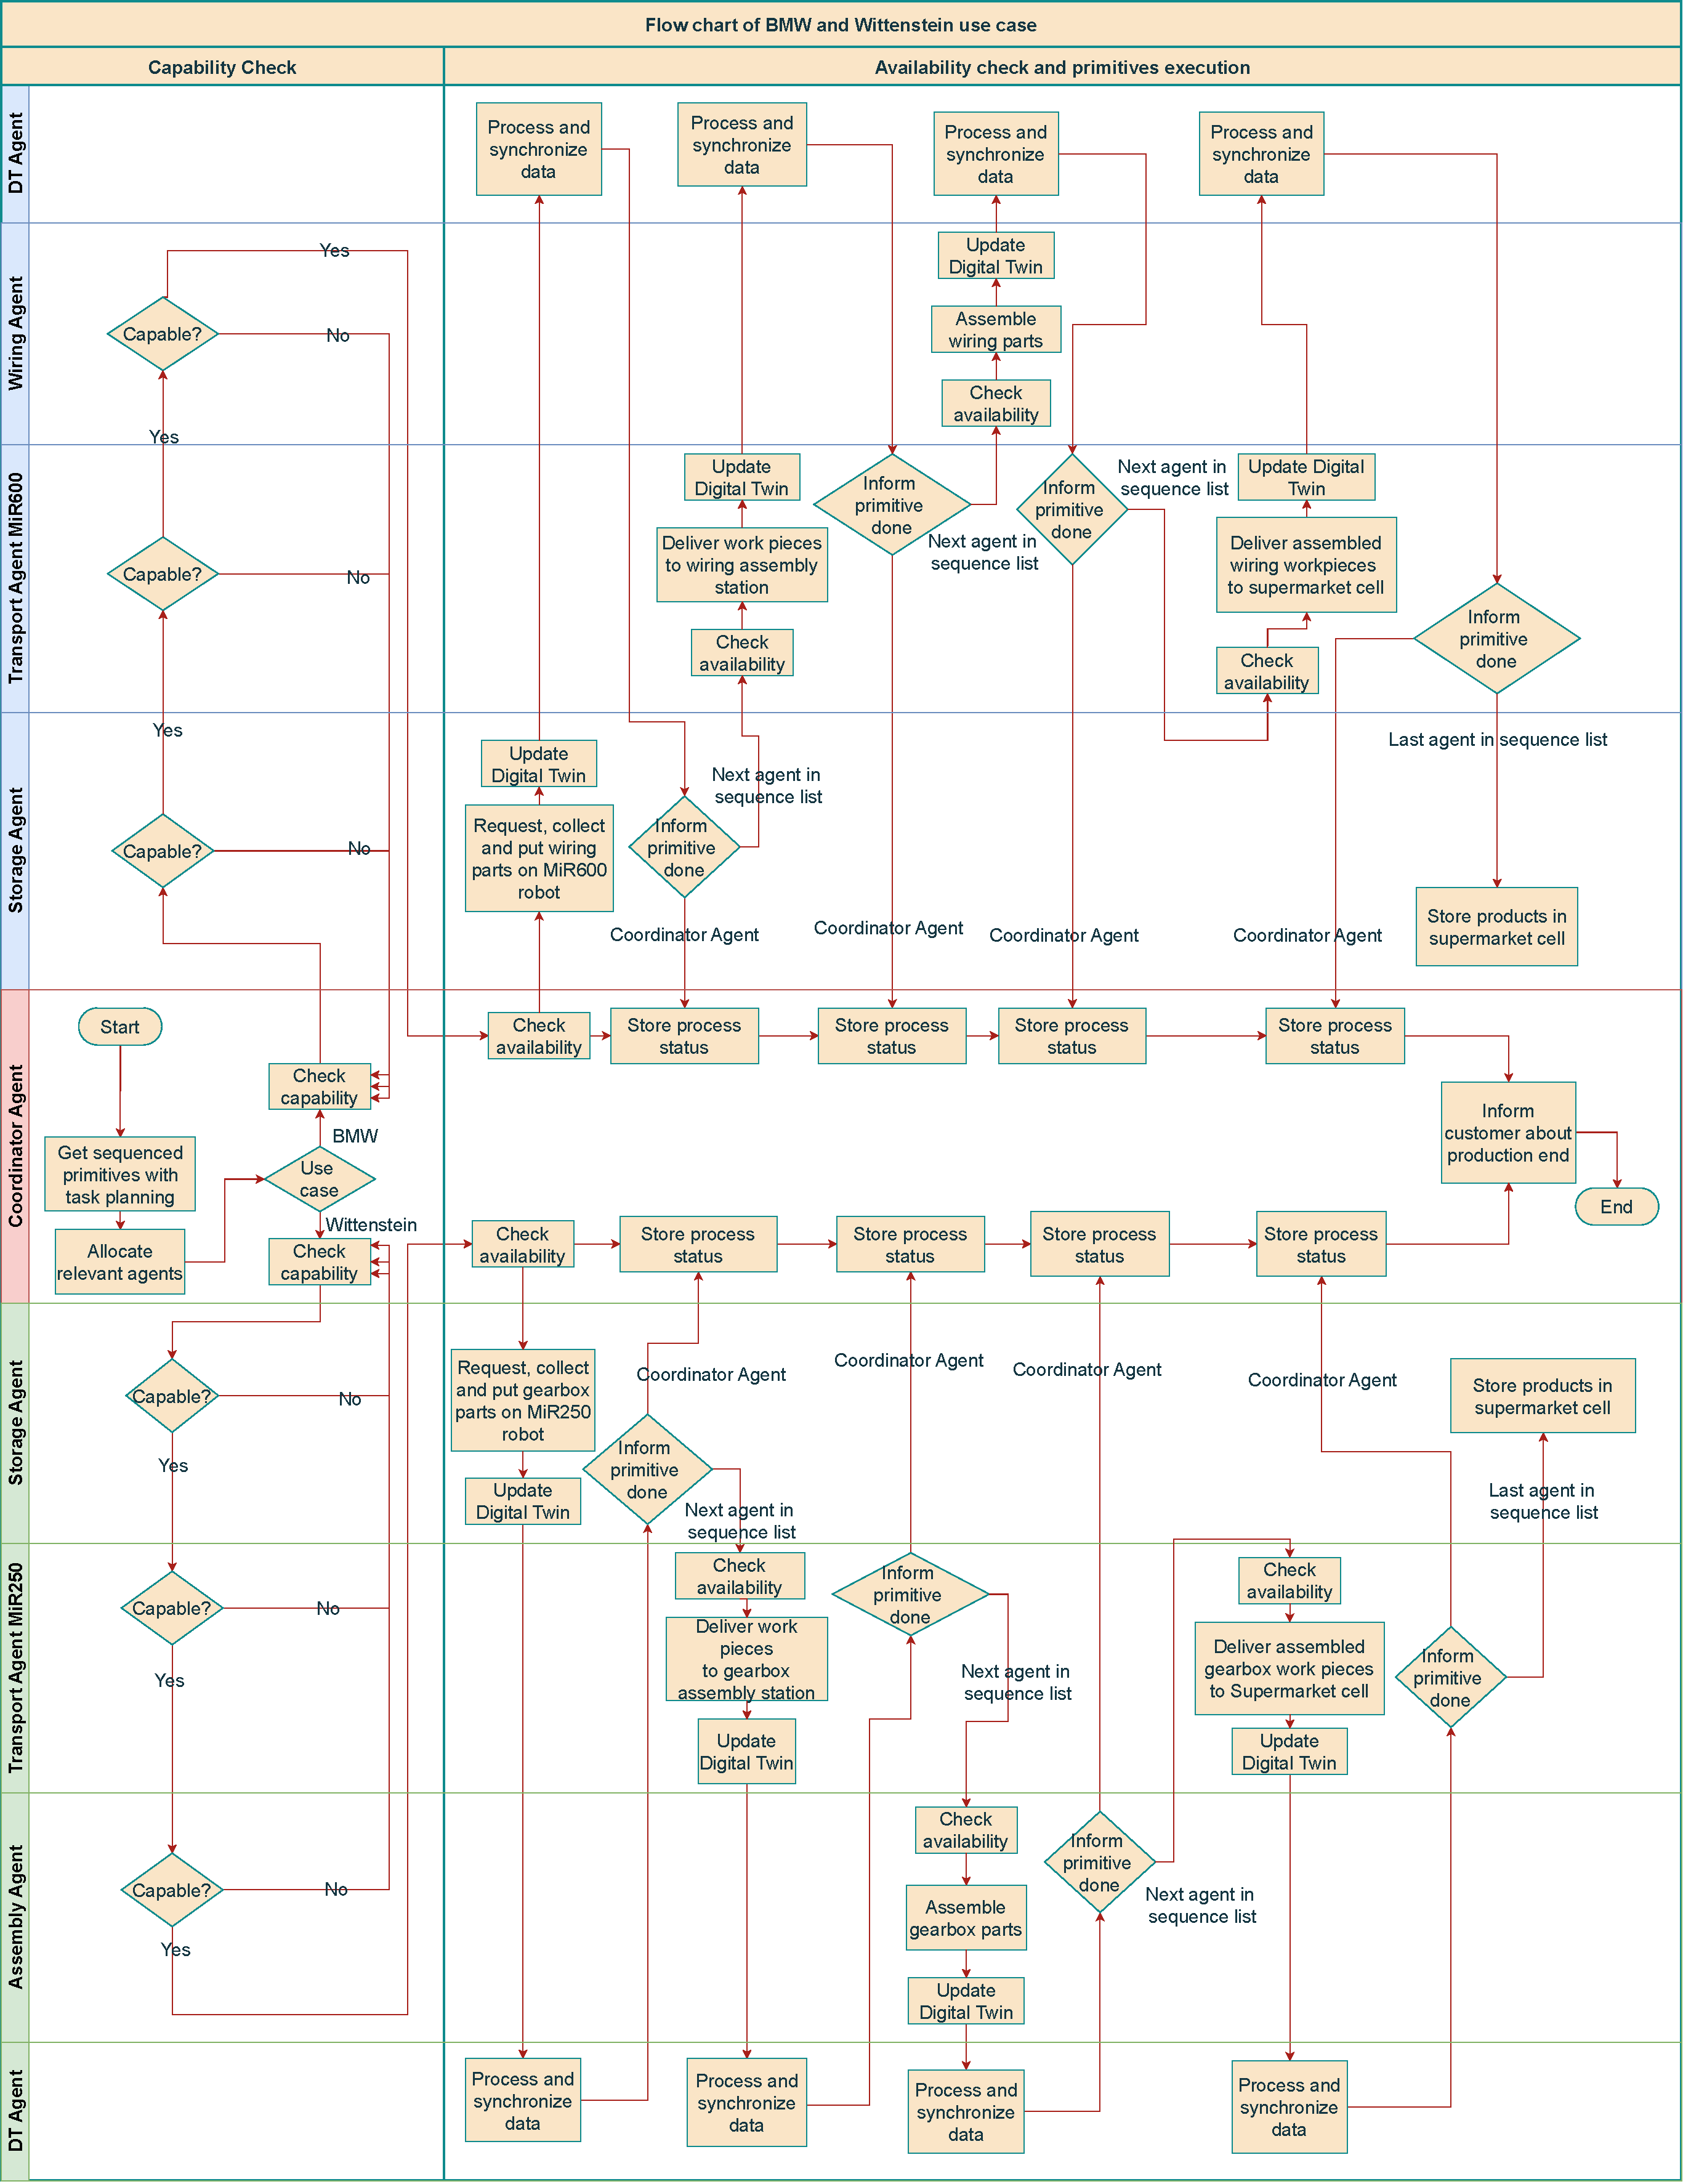
\includegraphics[width=\textwidth]{figures/tests/usecase/Usecase_flow.pdf}\hfill 
    \caption{Flowchart of BMW and Wittenstein use case of the \gls{mas} architecture. 
    Blue containers: BMW use case, allocated agents are Storge agent, 
    Transport agent MiR600, Wiring agent and Digital Twin agent respectively. 
    Green Containers: Wittenstein use case, allocated agents are Storage agent, 
    Transport agent MiR250, Assembly agent and Digital Twin agent respectively. 
    Red container: \gls{cda} for both usecases.} 
    \label{fig: Flowchart-usecase}
\end{figure}
The primitives, agents and execution sequence for both BMW and Wittenstein use cases 
are predefined. However, only the timing behaviors of the BMW use case are tested due 
to similarity. The average \gls{rtt} and WebSocket data transmission time of the BMW 
use case are presented in Table \ref{tab: mean-usecase-time}. The test was conducted 
100 times, but the number of messages exchanged among agents varied greatly. Therefore, 
the test results and average values can only be used as a reference to understand the 
data transmission process in actual production. In order to provide a more detailed data 
distribution of each message, the violin plot in fig.\ref{fig: violin-CDA-T600} is 
presented along with other test results with other agents (see fig.\ref{fig: violin-CDA-ST} to \ref{fig: violin-T600-WI}). 
Based on these results, it can be concluded that the message transport in the system meets 
the real-time requirements, with the largest message size of 636 Bytes taking a maximum of 
10ms and the smallest taking about 0.2ms.


\begin{table}[htbp]
    \small
    \centering
    \caption{Average delays between agents with different string message length and 
    different amount of messages.}
    \label{tab: mean-usecase-time}
    \begin{tabular}{|m{0.13\textwidth}|m{0.17\textwidth}|m{0.17\textwidth}|m{0.17\textwidth}|m{0.17\textwidth}|}
    \hline
    \multicolumn{5}{|c|}{\textbf{Average delays between agents (RTT/Transmission time)}}                                                            \\ \hline
    \textbf{}                         & \textbf{Coordinator Agent}             & \textbf{Storage Agent}        & \textbf{Transport Agent MiR600}    & \textbf{Wiring Agent}\\ \hline
    \textbf{Coordinator Agent}      & None                  & 1.029355ms /0.820172ms & 1.067170ms /0.849335ms  & 1.032151ms /0.817049ms \\ \hline
    \textbf{Storage Agent}          & 0.998253ms /0.794590ms & None                  & 1.427890ms /1.158142ms  & None                  \\ \hline
    \textbf{Transport Agent MiR600} & 1.055389ms /0.840291ms & 1.422970ms /1.150696ms & None                   & 1.668750ms /1.344250ms \\ \hline
    \textbf{Wiring Agent}           & 0.988012ms /0.783014ms & None                  & 1.654000ms /1.361000ms  & None                  \\ \hline
    \end{tabular}
\end{table}


\begin{figure}[htb]
    \centering
    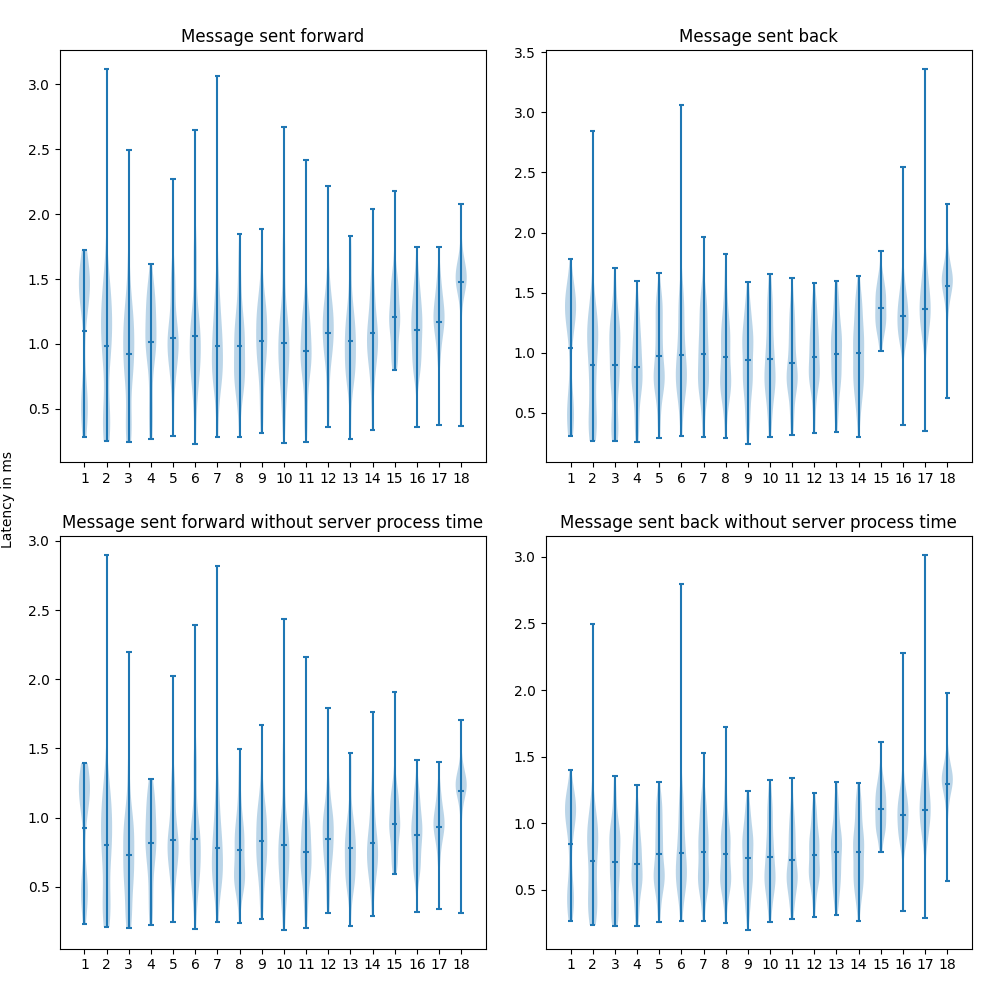
\includegraphics[width=\textwidth]{figures/tests/usecase/violin_CoordinatorAgent_to_TransportAgent_MiR600.png}\hfill 
    \caption{Test to measure \gls{rtt} and transmission time between \gls{cda} and 
    TransportAgent\_MiR600 for 100 times. The number in x-axis respresents the 
    corresonding messages. \protect\ref{firstfootnote}}
    \label{fig: violin-CDA-T600}
\end{figure}

%addtional for footnote in caption
\footnotetext[2]{\label{firstfootnote}https://github.com/XuezhouHou/Websocket\_MAS/new\_MAS/output/plots/table4UCBMW.xlsx}



\section{External}\label{chap: Result-External}
As for the delay measurement of the external \gls{dta} system, tests for the 
upload and download are done separately, with different packet sizes as tuning 
parameters. 


\subsection{Test results of data transmission 
time in \gls{tcp} sockets between robots and \gls{dta} across 
various packet lengths} \label{chap: Result-RCP-DTA}

To better measure the influence of different packet lengths on transmission time from 
a \gls{rcp} to \gls{dta} utilizing \gls{tcp} sockets, the packet length of JointGripper 
(joint and gripper of the robot arm) position values should be larger than that of the 
Elbow (elbow of the robot arm), they are 151 and 80 Bytes respectively. As depicted in 
fig.\ref{fig: SR-JointGripper-Elbow}, the mean transmission time of JointGripper is 
larger than Elbow, which verifies that larger files take longer to transfer. 
The cumulative delays of both data lengths also show a linear growth relationship in 
the upper graph, which means there are no major fluctuations or irregularities in 
transmission speeds or times for the packets in \gls{tcp} sockets. 


\begin{figure}[htb]
    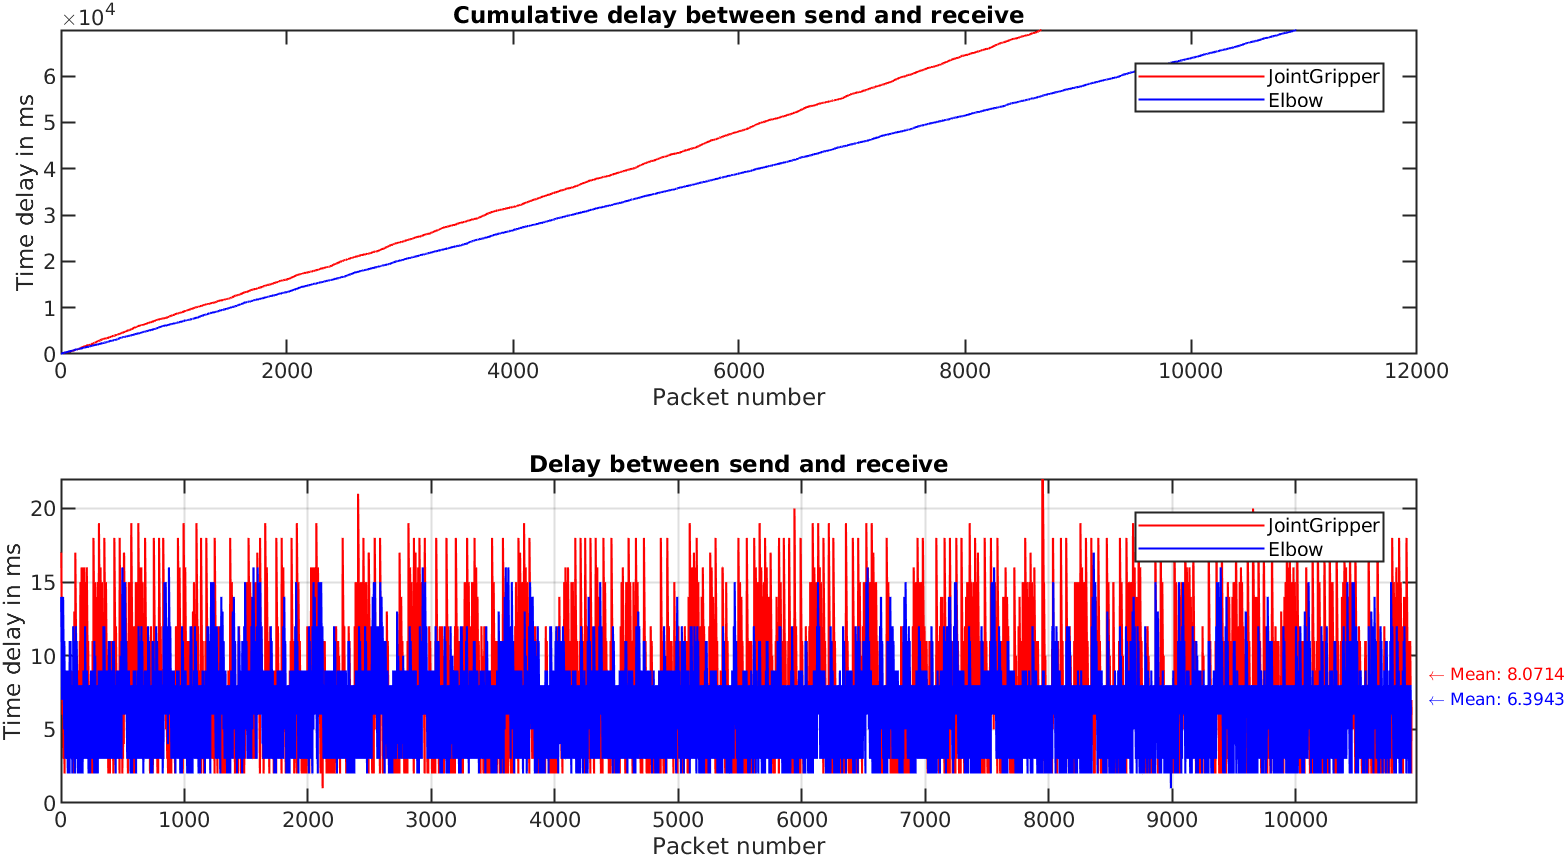
\includegraphics[width=\textwidth]{figures/tests/DT/Delay_SendReceive_JointGripper_Elbow.png}
    \centering
    \caption{Tests for different packet sizes w.r.t data transmission time between robots 
    and \gls{dta}. \label{fig: SR-JointGripper-Elbow}}
\end{figure}

Since each packet only takes a few milliseconds to be transported, the real-time 
requirement for production processes is again fulfilled. 



\subsection{Test results of data transmission time in \gls{tcp} sockets between \gls{dta} 
and \gls{ms} Azure Digital Twin platform across various packet lengths} \label{chap: Result-DTA-DT}

However, in the program, the most considerable variance 
the total data transmission time is the \gls{rtt} from local devices to the global digital 
twin. In addition to the \gls{rtt}, the data upload and download time is also measured 
separately, which has an opposite result as those from the other research\cite{cainelli_performance_2023}. 
In the paper, the resulting uplink data transmission time is larger than the downlink 
data transmission time. The difference between both tests is the research team from 
Magdeburg measured delay with logical links from a 5G standalone network and the industrial 
5G devices. In contrast, our test was based on data update times in the cloud. The latency 
between data upload and update reflects the actual digital twin data update patterns, 
which includes additional process time in the cloud. Therefore, we can infer that the 
increased latency of data upload may be caused by the internal Azure Digital Twin Model 
API for data update (an unclosed issue in \gls{ms} Q\&A\footnote{https://learn.microsoft.com/en-us/answers/questions/1328803/experiencing-slow-load-times-on-azure-digital-twin}).
    

It is worth mentioning that the data upload time from JointGripper and Elbow has little to 
no difference since the upload mechanism of Azure Digital Twin is limited by sending twin 
values one after one. There is only such function to update up to one twin simultaneously. 
In order to differentiate the upload speed, the patch size of the to-be-updated twin values 
should vary. The fig.\ref{fig: UD-cycle-JointGripper} again shows the cumulative delays 
with the same conclusion as in fig.\ref{fig: SR-JointGripper-Elbow} and mean \gls{rtt} is 
slightly lower than 100ms, which is still under the real-time requirements. The packet for 
upload and download will be routed to the cloud, which not only goes through the internal 
5G network but also the internet externally, which results in much higher latency. Compared 
with the test results from \cite{cainelli_performance_2023}, optimizing the internal twin 
update mechanisms can further reduce data \gls{rtt}. 


\begin{figure}[htb]
    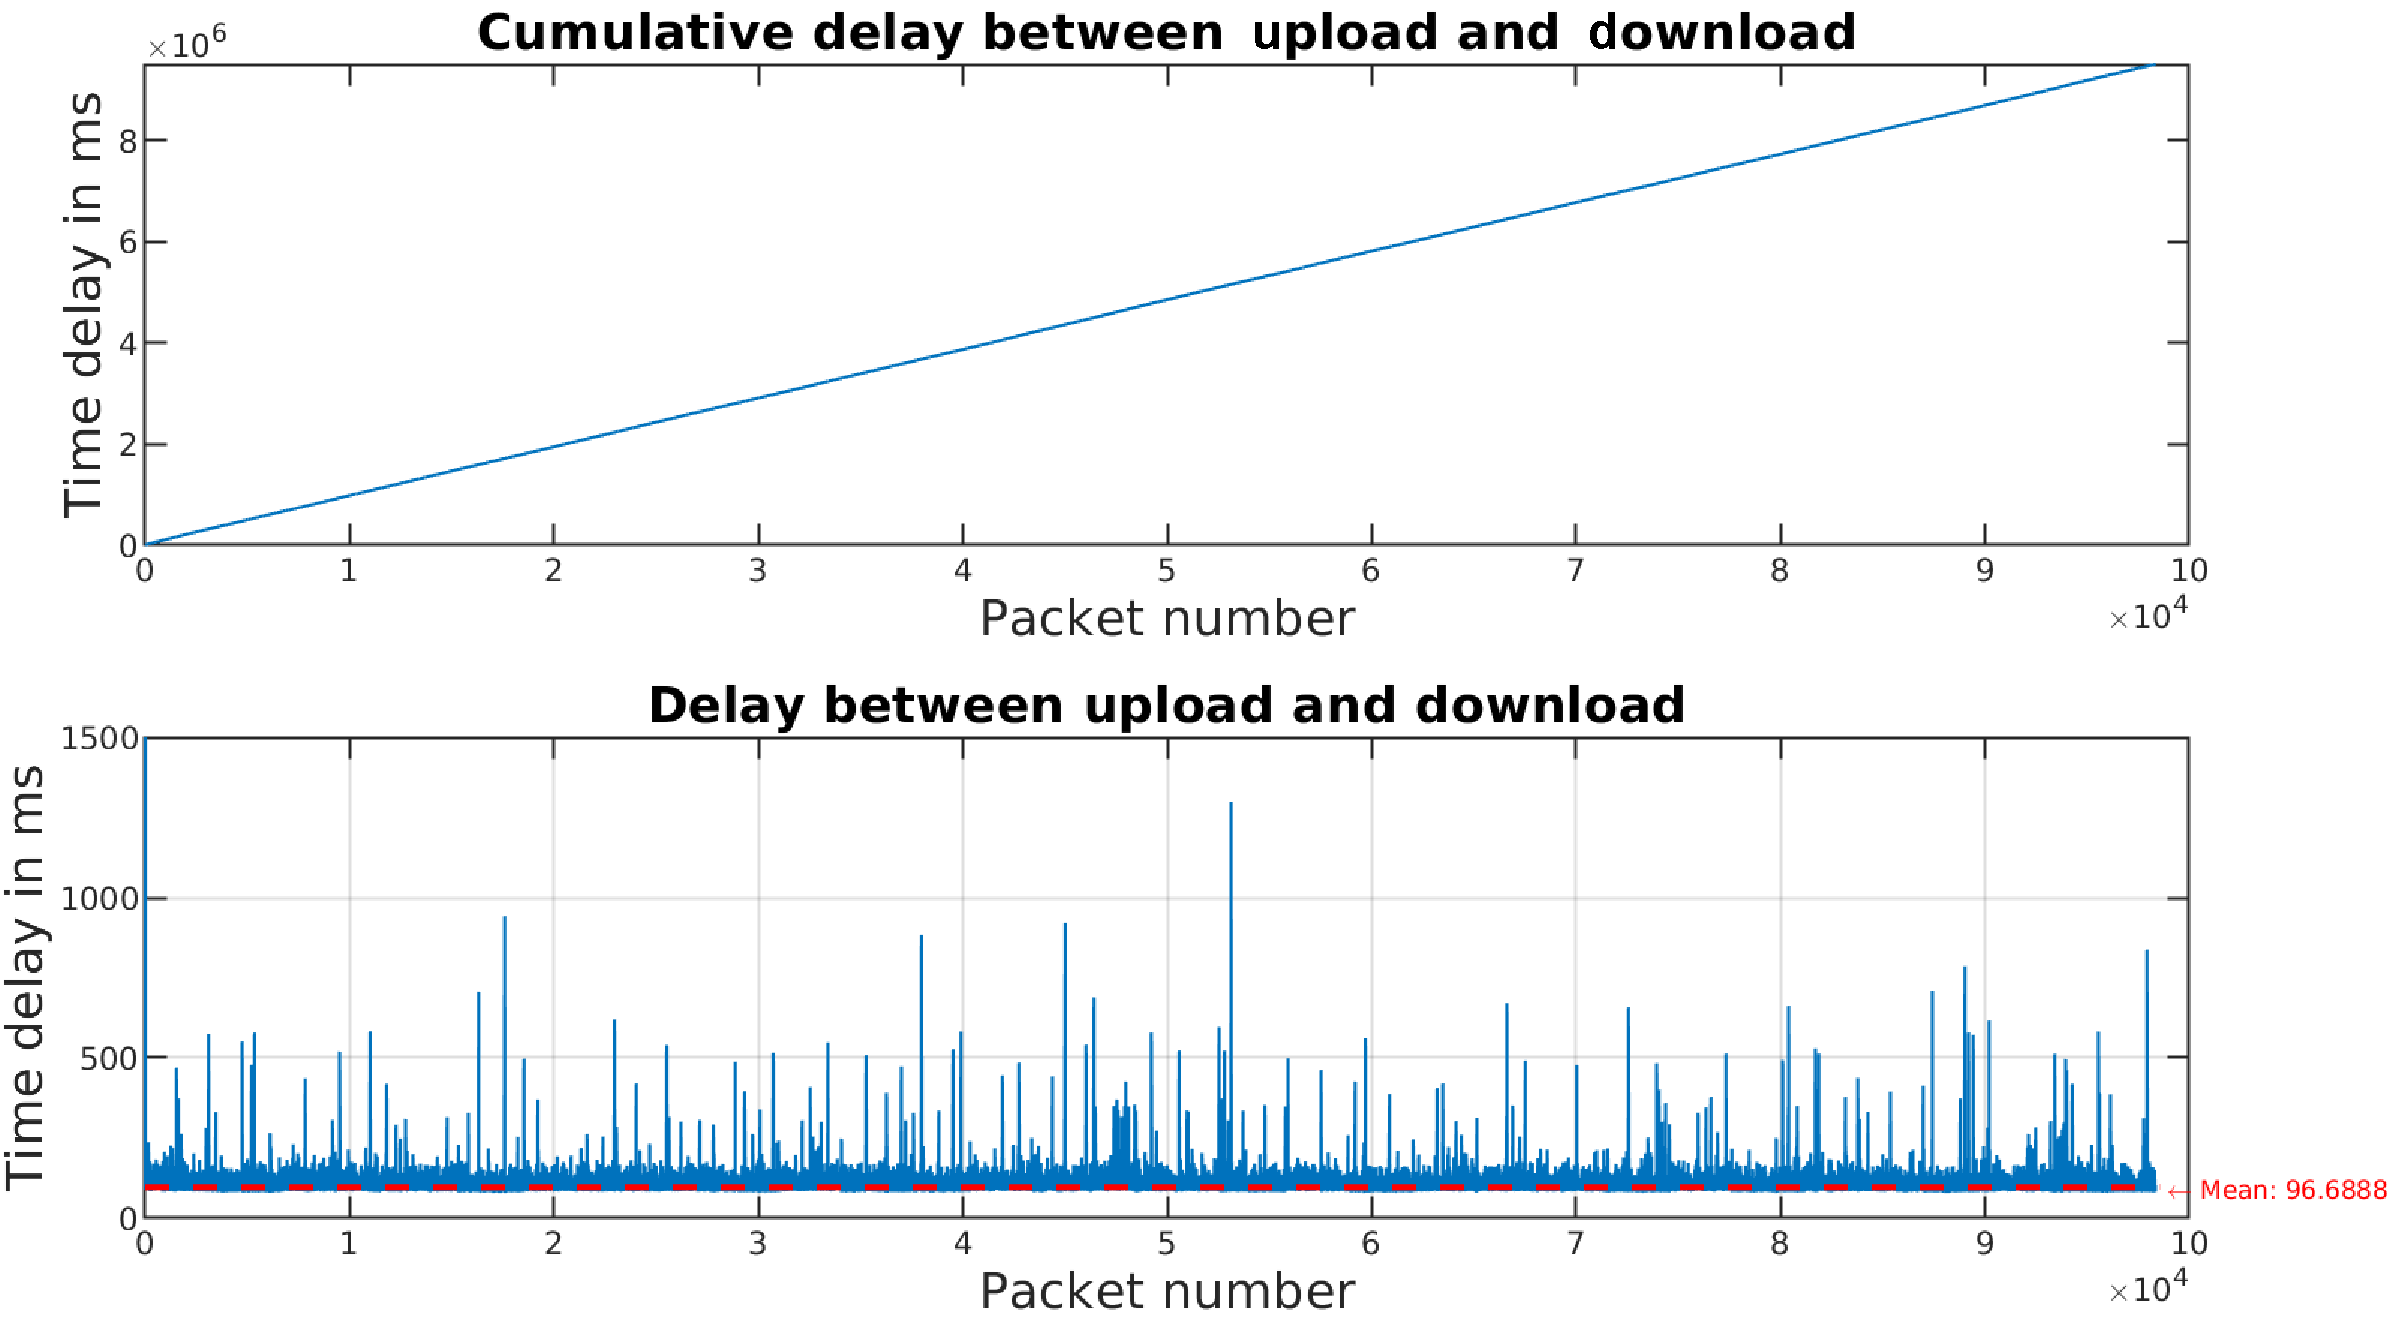
\includegraphics[width=\textwidth]{figures/tests/DT/Delay_UploadDownloadCycleTime_JointGripper.pdf}
    \centering
    \caption{Tests for \gls{rtt} of data upload and download for JointGripper. \label{fig: UD-cycle-JointGripper}}
\end{figure}

As mentioned, the data upload time is larger than the download time, as depicted in 
fig.\ref{fig: UD-sep-JointGripper}. The average upload time of JointGripper values is under 30ms, 
while the download time results in about 70ms. Under the same conditions, the differences 
between JointGripper and Elbow in both values for are negligible with only 1-2ms difference (see \ref{chap: append-DTagent} fig.\ref{fig: UD-cycle-Elbow} 
and \ref{fig: UD-sep-Elbow}), due to the one after one twin upload mechanism. However, 
the time spent connecting to the Digital Twin platform needs to be factored in 
as well, which takes about 9400ms for JointGripper and 9600ms for Elbow. Although it 
does not fulfill the real-time requirement, it is still counted for comparison 
to the average download time.




\begin{figure}[htb]
    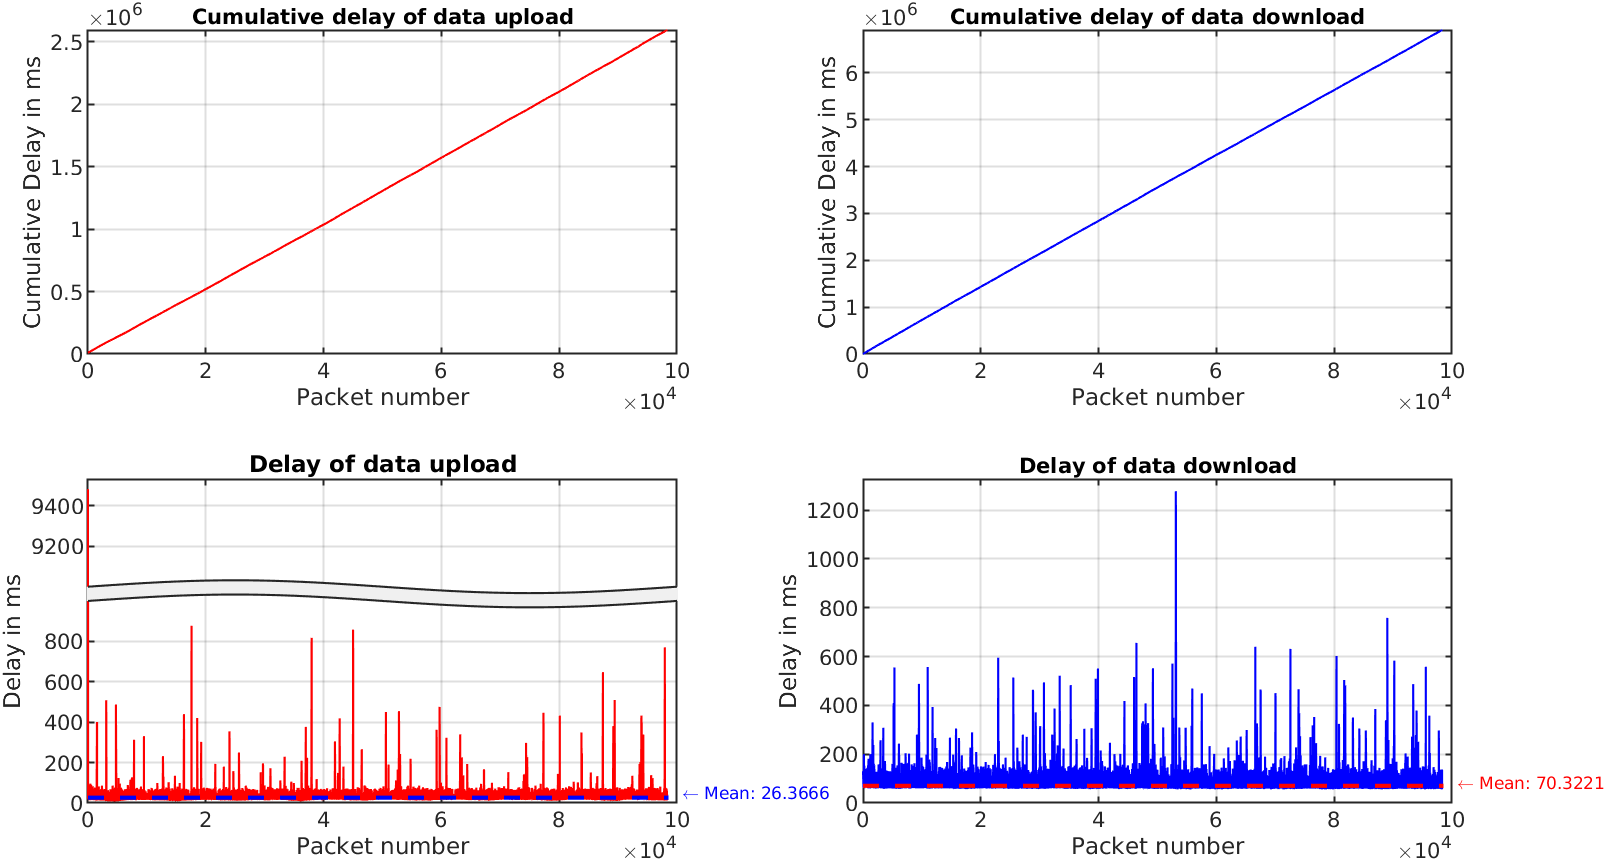
\includegraphics[width=\textwidth]{figures/tests/DT/Delay_UploadDownload_JointGripper.png}
    \centering
    \caption{Tests for delays between \gls{dta} and digital twin update of JointGripper, 
    and delays for twin value download. \label{fig: UD-sep-JointGripper}}
\end{figure}


To differentiate the upload speed based on packet size, two patches with 
different sizes are introduced. Ideally, the small data patch with a size of 
49 Bytes should induce a higher transmission speed than the large one with 554 Bytes, 
but the reality is quite different. The test results of all the 
delay measurements for both patch sizes are presented as a violin plot in 
fig.\ref{fig: UD-violin-patchsize}. As expected, the upload time of large 
patches is more than that of small patches, while the result of download time is 
the opposite. This results in nearly identical total \gls{rtt} of both. 
The reasons can be that each test is done at a different time, which results in a 
fluctuation related to the network traffic, cloud service loads, amount of end users 
under the same 5G network, and many more, which influence the data transmission time 
even more than the patch sizes.

\begin{figure}[htb]
    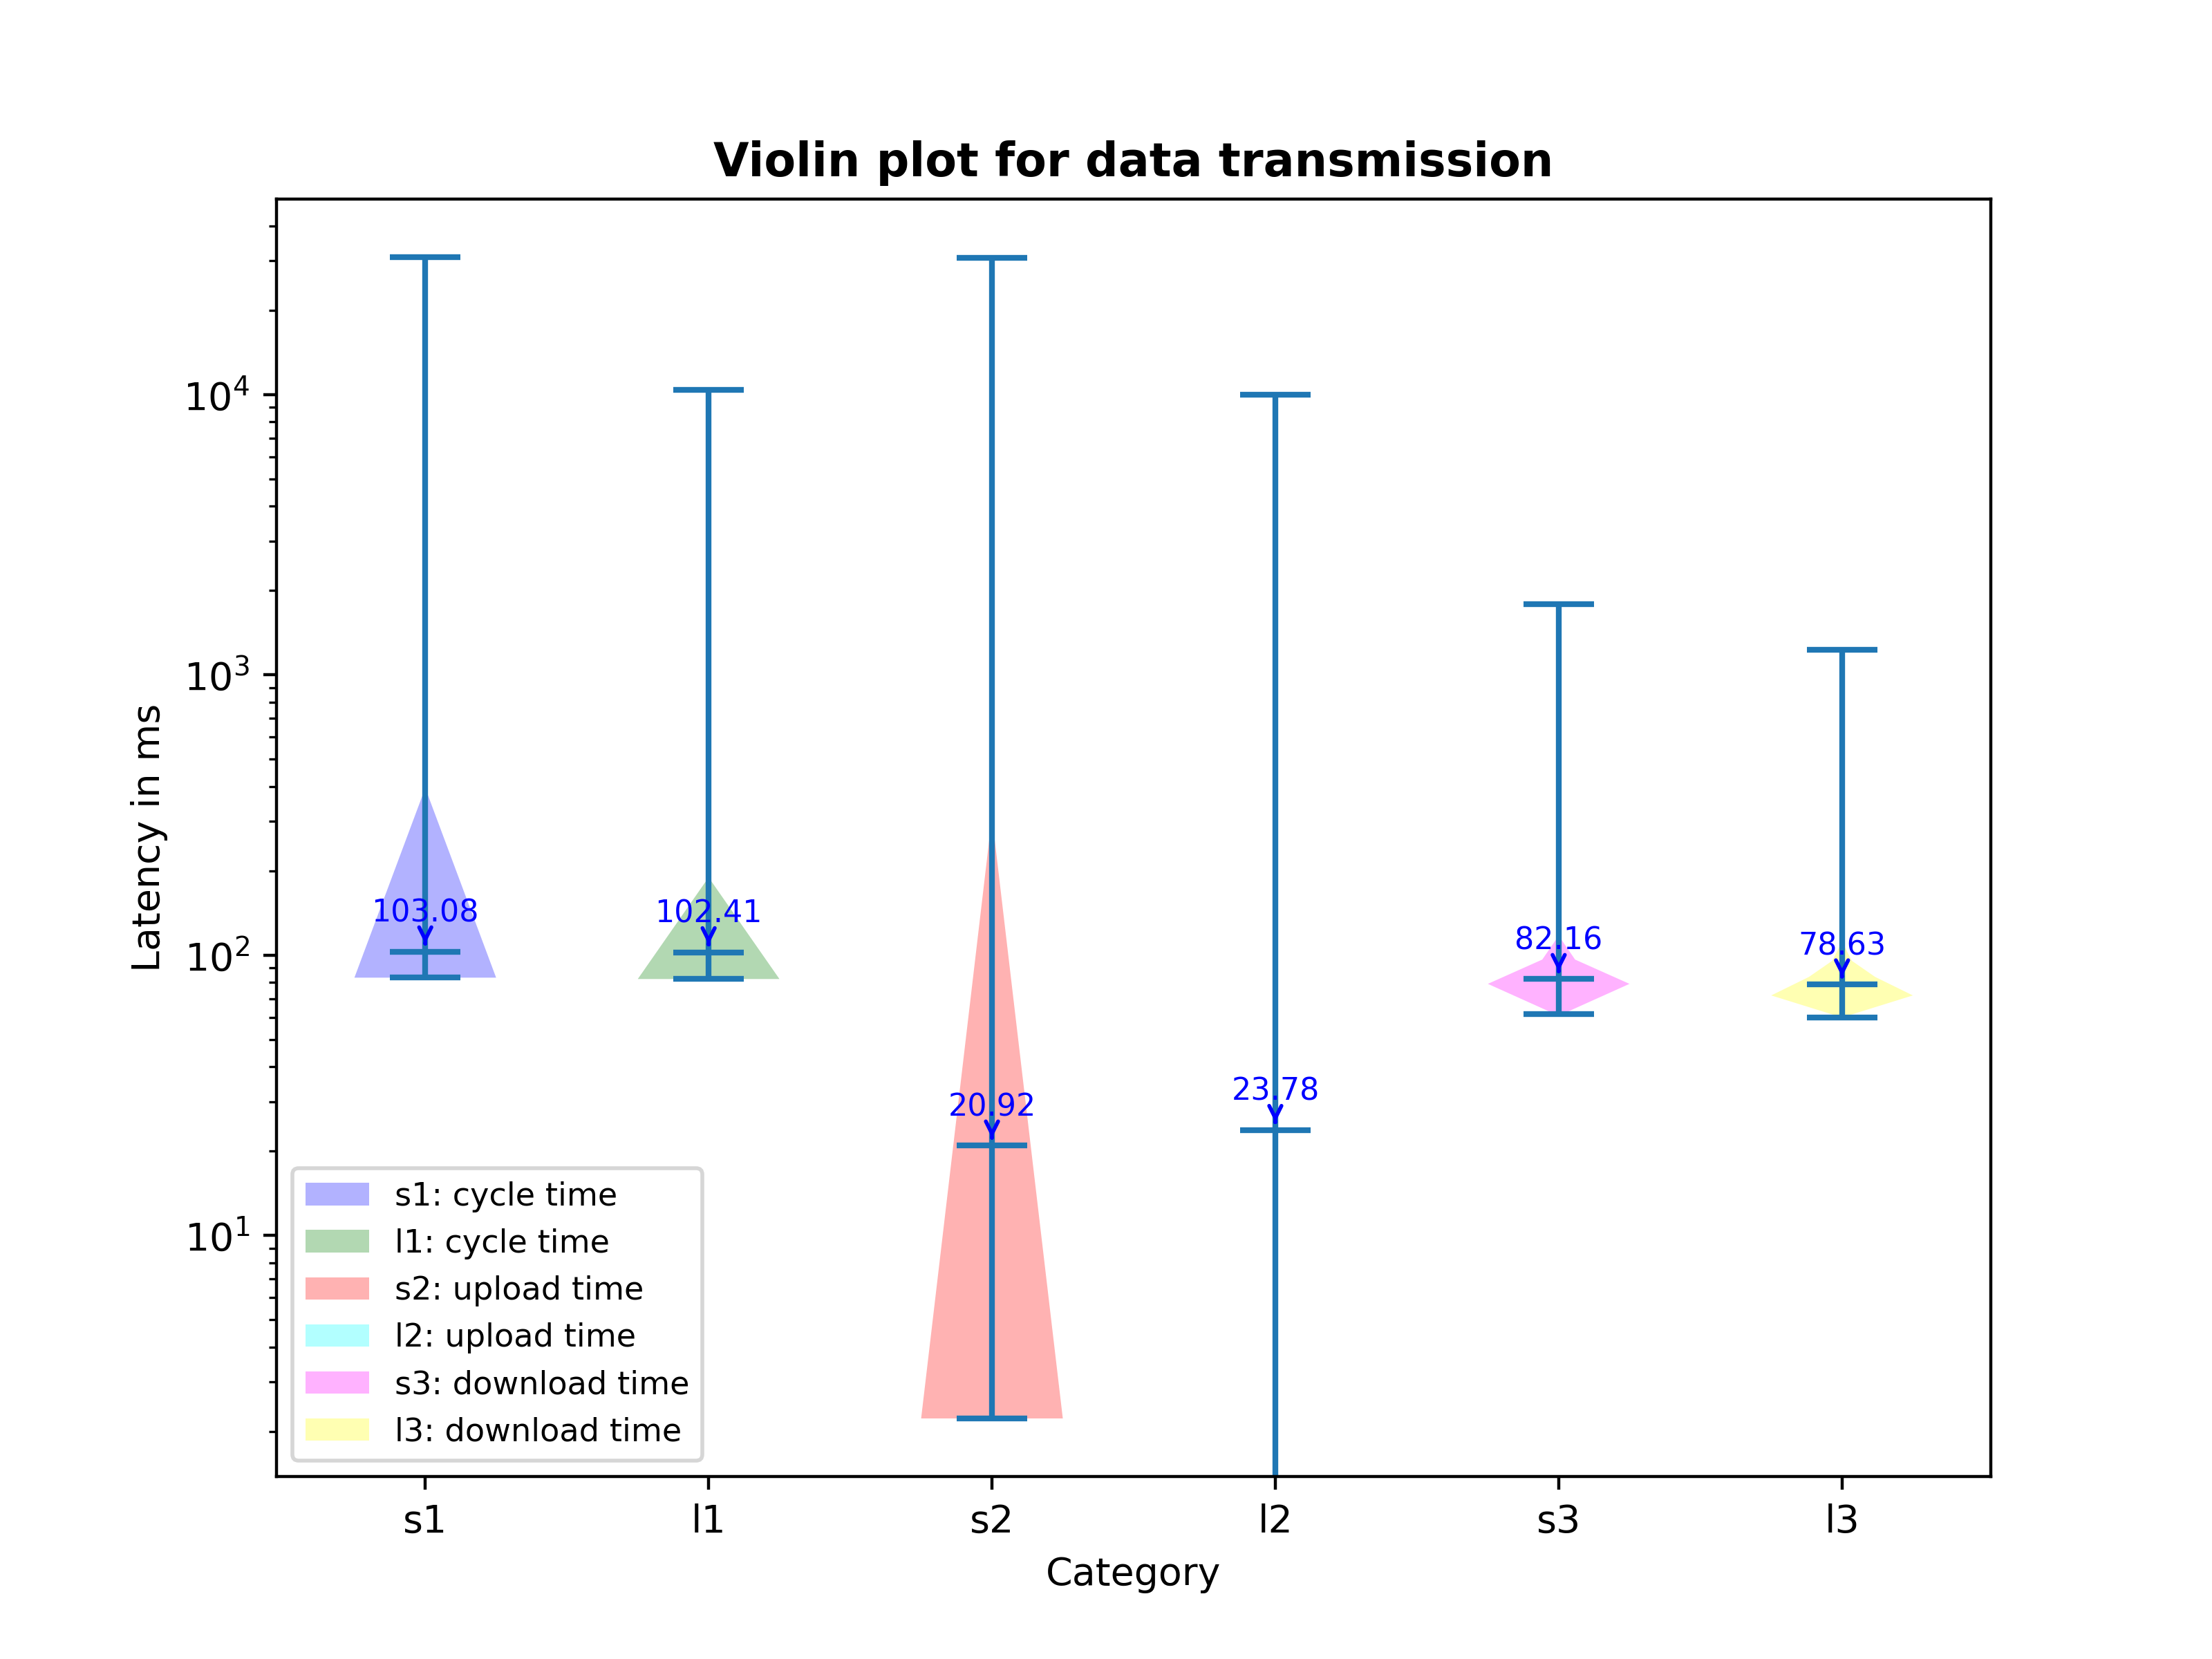
\includegraphics[width=\textwidth]{figures/tests/DT/violin_patch_size.png}
    \centering
    \caption{Tests for \gls{rtt}, delays between \gls{dta} and digital twin 
    update of JointGripper, and delays of twin value download for 
    two different patch sizes. In the graph, s represents small patches 
    and l for large patches.\label{fig: UD-violin-patchsize}}
\end{figure}

In general, the data upload and download time between \gls{dta} and the cloud is 
much higher than the field-level data transmission time under \gls{tcp} sockets. 
A fig.\ref{fig: SR-U-D-violin} shows the variance and mean of those in a violin plot 
for a more intuitive observation. 
Compared to the violin plot in fig.\ref{fig: UD-violin-patchsize}, the send and receive 
processes always show a symmetric triangular shape, suggesting a limited sample size. 
Considering the non-symmetric triangular shape of the uploading and downloading processes, 
it is likely to be attributed to the data points with a predominance at the lower extremum 
and the minimal presence at the upper extremum.
\begin{figure}[htb]
    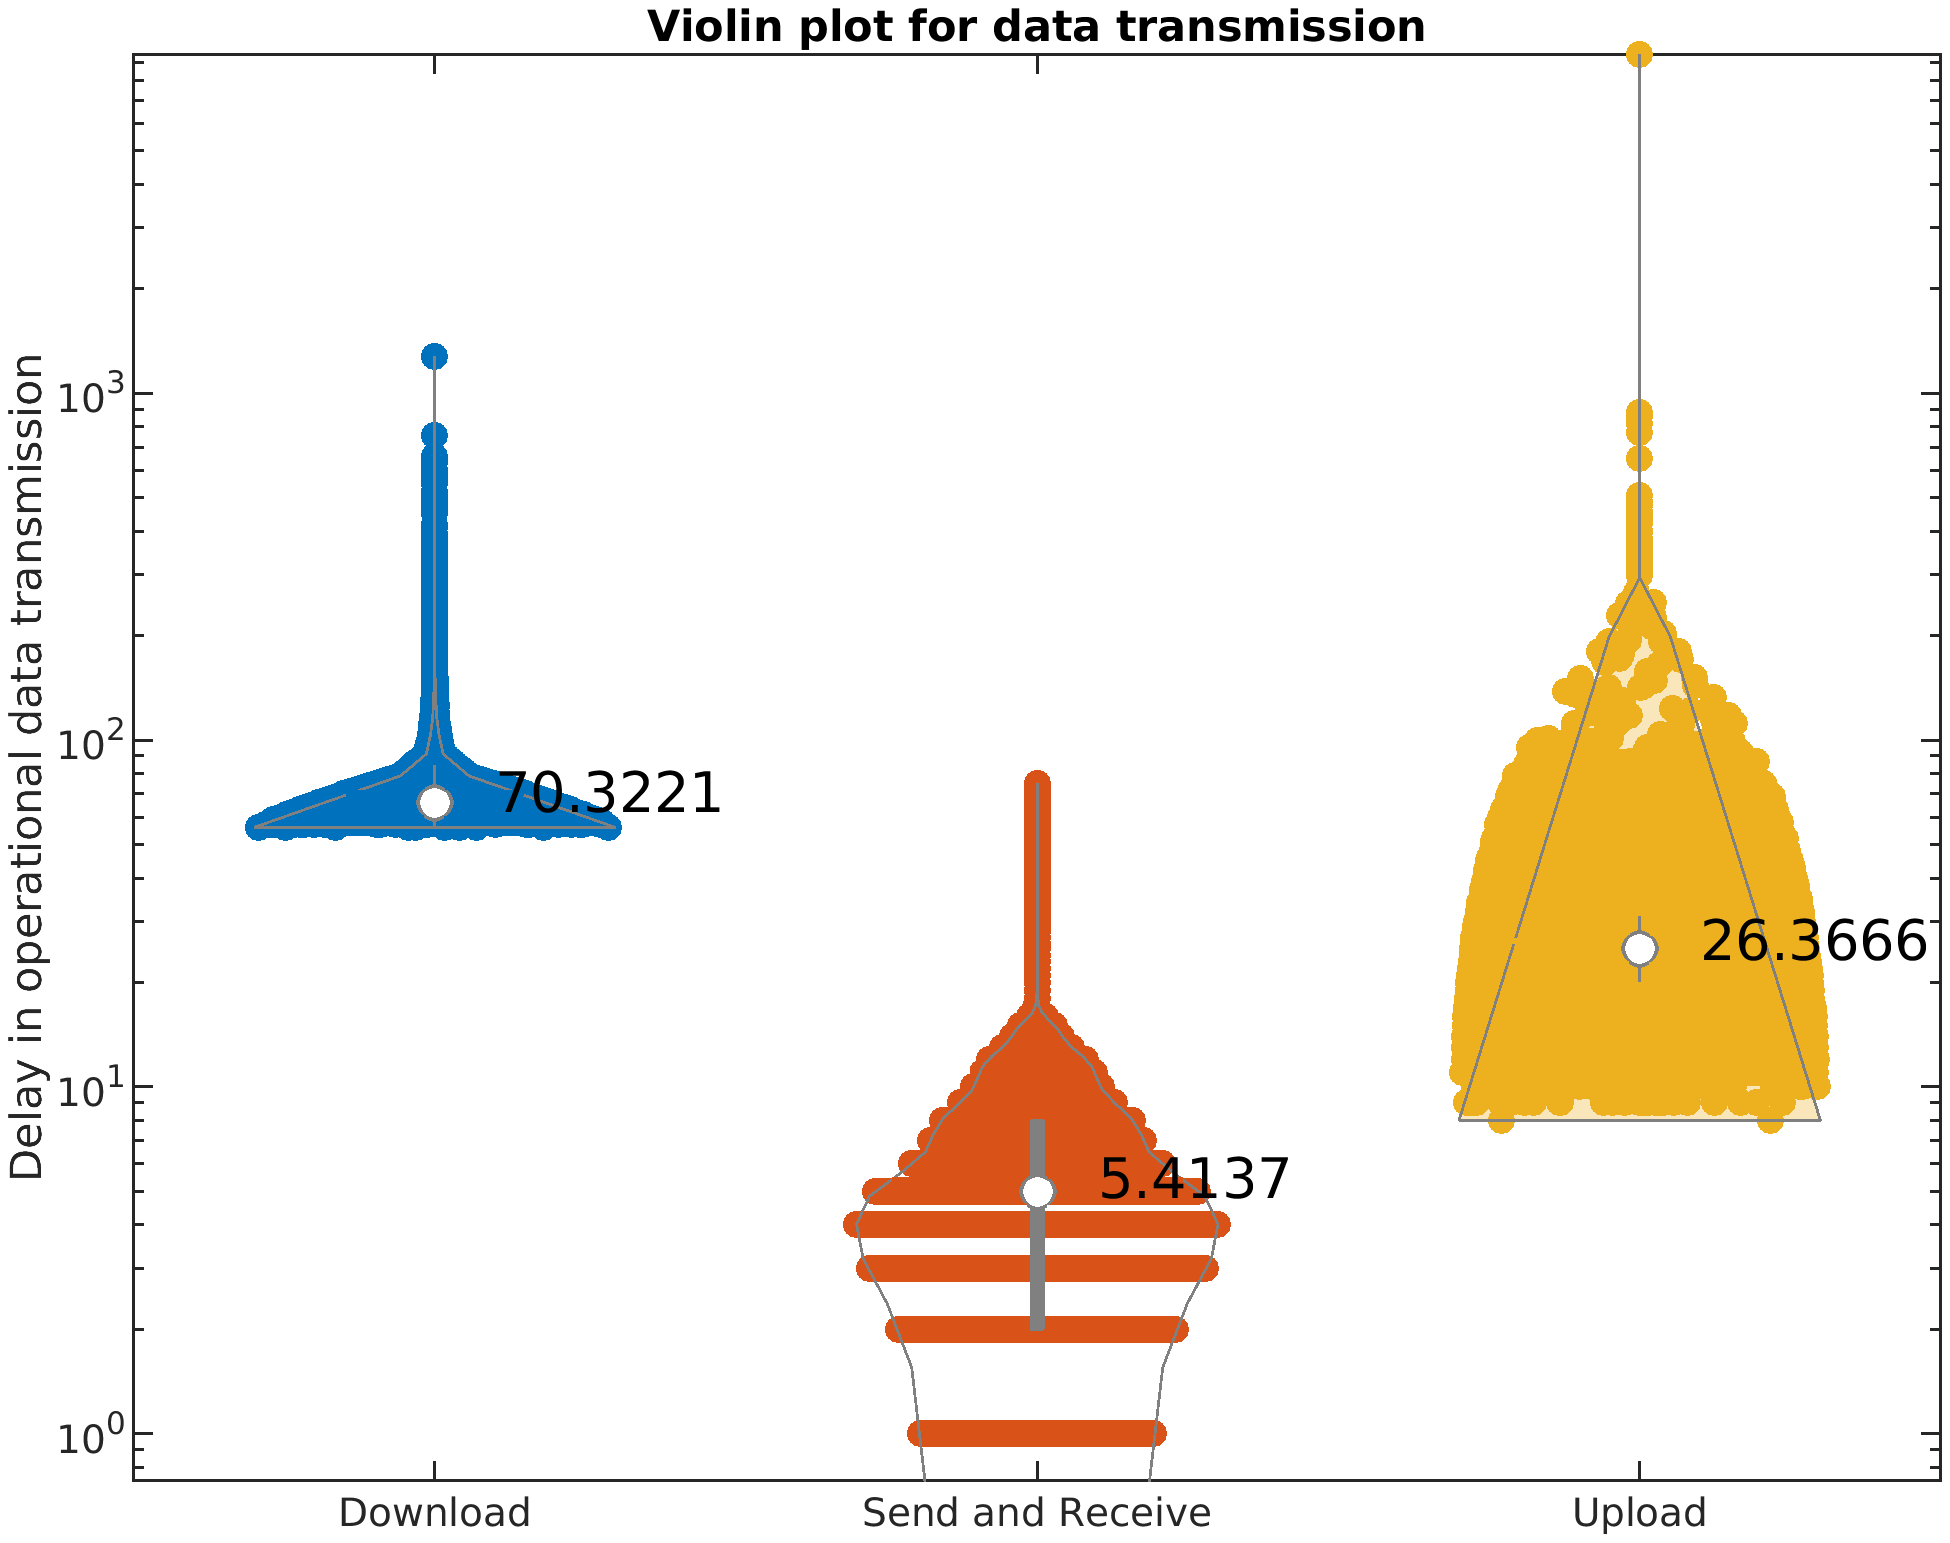
\includegraphics[width=\textwidth]{figures/tests/DT/log_violin_Plot_3cat.png}
    \centering
    \caption{Tests for data transmission time from robot to \gls{dta}, 
    delays between \gls{dta} and digital twin 
    update of JointGripper, and delays for twin value download.\label{fig: SR-U-D-violin}} 
\end{figure}

